%!TEX program = xelatex
%\documentclass[cn,12pt,math=newtx,citestyle=gb7714-2015,bibstyle=gb7714-2015]{elegantbook} 
\documentclass[12pt]{book}

%%%%% setting for environments%%%%%%%%
\usepackage{geometry} %page setting 
\geometry{a4paper,left=2.6cm,right=2.6cm,top=1.8cm,bottom=1.8cm}
\usepackage[cache=false]{minted} % formate the latex language in latex code with some special characterize.
%\usepackage{elegant} % This package of sty file, which lay the fold,  is found on internet and added to this project.
\usepackage{hyperref} %% Insert the link for latex.
\usepackage{elegant}

%%%%setting for fonts%%%%%
\usepackage{xeCJK}
\setmainfont{Times New Roman}
\usepackage[fontset=macnew]{ctex} %This package used for texstudio in mac.
\usepackage{fontspec}
\usepackage{metalogo} % latex logo

%%%%%%%%%%%setting for tables%%%%%%%%%
\usepackage{listings} % code in example
\usepackage{rotfloat} %sidewaystable and sidewaysfigure 
\usepackage{array}
%\usepackage{multicol} % table
\usepackage{multirow}
\usepackage{longtable}
%\usepackage{tabularx}
%\usepackage{ltablex}


%%%%%%setting for math%%%%%%%%%%%%
\usepackage{amsmath}
\usepackage{cases}

%%%%%%%%%%%setting for figures%%%%%%%%%
\usepackage{graphicx}
\graphicspath{{./figure/}} %%%%% path should be include in '{}'
\usepackage{autobreak} % for too long line,autobreak it.
%\usepackage[figuresright]{rotating}
\usepackage[inkscapelatex=false]{svg} % insert svg file
\svgsetup{inkscapeexe=/opt/homebrew/bin/inkscape}

%\title{科技论文写作排版}
\title{\LaTeX{} Writing}
%\subtitle{\LaTeX{} 经典之作}

\author{Kang Yun}
%\institute{Elegant\LaTeX{} Program}
\date{May 2, 2021}
%\version{0.1}
%\bioinfo{自定义}{信息}

%\extrainfo{各人自扫门前雪,休管他人瓦上霜。—— 陈元靓}

\setcounter{tocdepth}{3}

%\logo{logo-blue.png}
%\cover{cover.jpg}

% 本文档命令
%\usepackage{array}
%\newcommand{\ccr}[1]{\makecell{{\color{#1}\rule{1cm}{1cm}}}}
%
%\definecolor{customcolor}{RGB}{32,178,170}
%\colorlet{coverlinecolor}{customcolor}

\begin{document}

\maketitle
\frontmatter

\tableofcontents

\part{\LaTeX{}科技论文排版}

\chapter{\LaTeX{}环境安装}

\section{Texlive}

\TeX{}是一种排版语言,通过命令来控制文档格式。\TeX{}在设计过程中采用了所思即所得的思想,与常见的文字排版工具Word相反。对于一些不熟悉命令行或缺乏计算机基础的人来说使用起来门槛过高,于是美国计算机学家莱斯利·兰伯特(Leslie Lamport)基于\TeX{}开发了扩展版\TeX{},即\LaTeX{}。与\TeX{}相比,使用者不需要高深的计算机知识和命令行操作方法也可以使用\LaTeX{}进行文档的排版工作。\LaTeX{}在数学公式方面的排版极为便利,尤其是在对一些复杂的表格和数学公式,也可以轻松完成。

\LaTeX{}作为一种排版语言,需要一个载体才能进行正常的工作。而让\LaTeX{}发挥作用的一个发行版本TexLive,目前来说是一种比较完成的持续维护更新的发行版本。对与未曾接触过\LaTeX{}的使用者来说是比较容易使用的一个工具。\LaTeX{}和TexLive之间的关系好比,C语言和C语言编译器之间的关系。没有编译器来对语言进行编译,机器便无法识别、工作。而在TexLive这个发行版本的编译器中来自带了一个简易的文本编辑器,可以用来完成一些简单的工作。

\section{Editor}

TexLive这个发行版中附带了一个功能相对简单的编辑器Texworks,该编辑器的界面相对简陋,对初次使使用者来说可以完成一些简单的不含复杂表格和数学公式的文档,但面对复杂的排版任务和以\LaTeX{}为主要排版工具的使用者来说,Texworks编辑器的使用起来略显不便,对与提高排版效率来说不是那么容易。于此同时,有Texstudiuo和Texmaker两款\LaTeX{}专用编辑器和vim、Sublime等兼容编辑器。

可以实现\LaTeX{}文档编写的软件较多,通常可以分为两类:可以实现texlive调用、编译的编辑软件,如Texstudio、Texworks、Emacs;通过插件来调用texlive实现编译的软件,如Vim、VScode等。texlive自带的Texworks编辑器轻量化,虽然功能上没有残缺,但是不适合打开较大的文件,且每个窗口只能打开一个tex文档,不便于结构化文档撰写和管理,同时界面过于简陋,对初学者的使用友好程度相对较低。VSCode虽然可以用来编写tex文档,但是其本身不是为编写tex文档而开发的,需要经过一番配置才可以运行,且软件本身过于庞大臃肿,不支持文档预览。Emacs和Vim两个强大的文本编辑器,经过一番配置之后,完全可以胜任\LaTeX{}的撰写和编译工作,但是这二者的入门学习成本相对较高。因此,重点介绍Texstudio编辑器。

\subsection{Texstudio}
TeXstudio是一款跨平台(Windows、Mac、Linux)的免费软件,用来编辑\LaTeX{}文档。TeXstudio软件针对\LaTeX{}设计了众多的快捷按键和便利的功能。例如:文件结构视图、代码补全和折叠、语法高亮和语法检查、行内实时预览和代码块、内置浏览等。TeXstudio对初学者入门\LaTeX{}完全够用,且学习的门槛相对较低。而非常熟悉\LaTeX{}的用户,可以在Texstudio软件内进行自定义宏,提高编写效率。Texstudio软件的下载途径:官网(目前很难访问),sourceforge(第三方的开源软件集合),\href{https://mirrors.tuna.tsinghua.edu.cn/github-release/texstudio-org/texstudio/}{清华大学的镜像}。

软件安装完成之后,用户仅需要做一点点设置工作:

1.用户根据自己的需要来设置显示语言和字体。读者可以根据自己的需要来设置语言和显示字体。如需要采用中文编写文件,则必须在option>Configure Texstudio 中,设置编译器为xeletex。如果在使用过成中用到了minted环境,则还需要在编译参数前添加一个选项:--shell-escape。

\begin{center}
     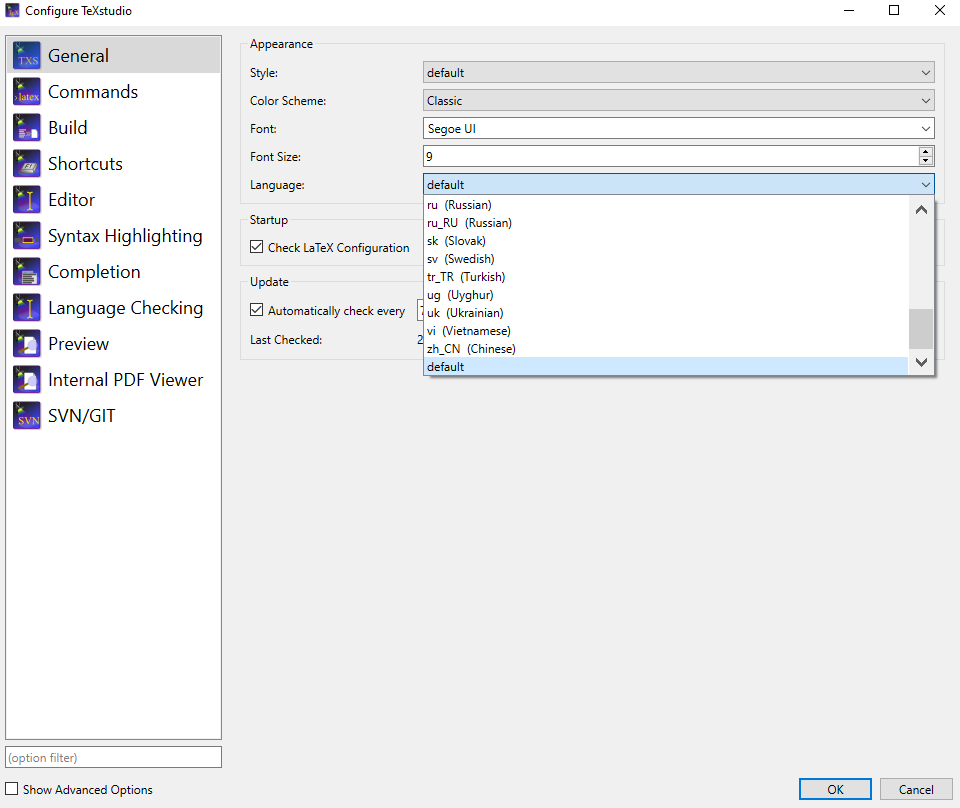
\includegraphics[scale=0.8]{./texstudio-lang.png}
\end{center}
2.根据排版的文字类型(中文或西文)来设置Texstudio在编译编译过程中调用的编译器类别:\LaTeX{}或xelatex。

\begin{center}
     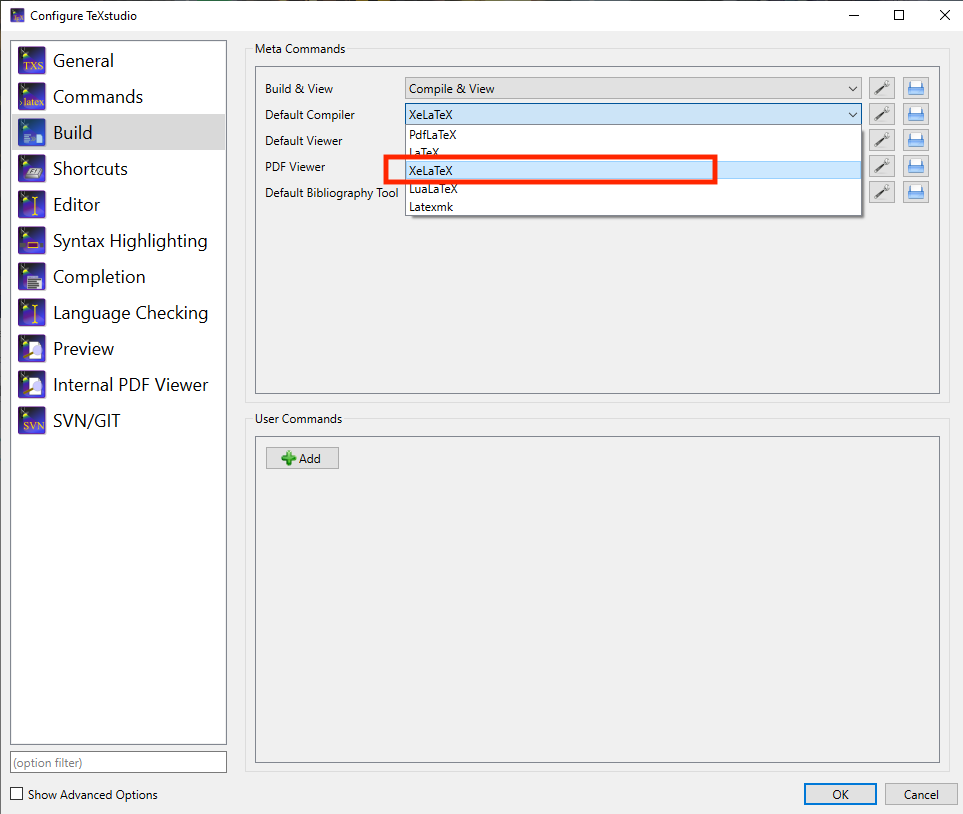
\includegraphics[scale=0.8]{./texstudio-build.png}
\end{center}
3.大多数情况下,用户不需要更改xelatex编译器的参数。但在用到minted环境时,需要在xelatex后补充参数`-shell-escape',即`xelatex.exe -shell-escape -synctex=1 -interaction=\\nonstopmopde \%.tex'。


\begin{center}
     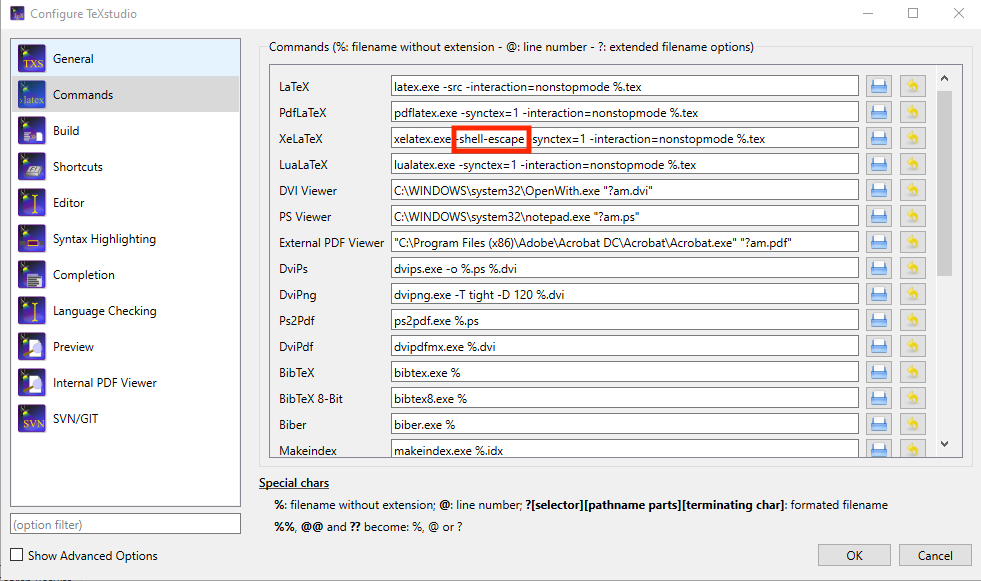
\includegraphics[scale=0.65]{./texstudio-command.png}
\end{center}
TeXstudio提供了语言拼写检查功能,用户可以自己从软件提供的跳转\href{https://extensions.libreoffice.org/}{链接},从libreoffice网站来下载相应语言的词典(词库),供软件进行拼写检查。


\begin{center}
     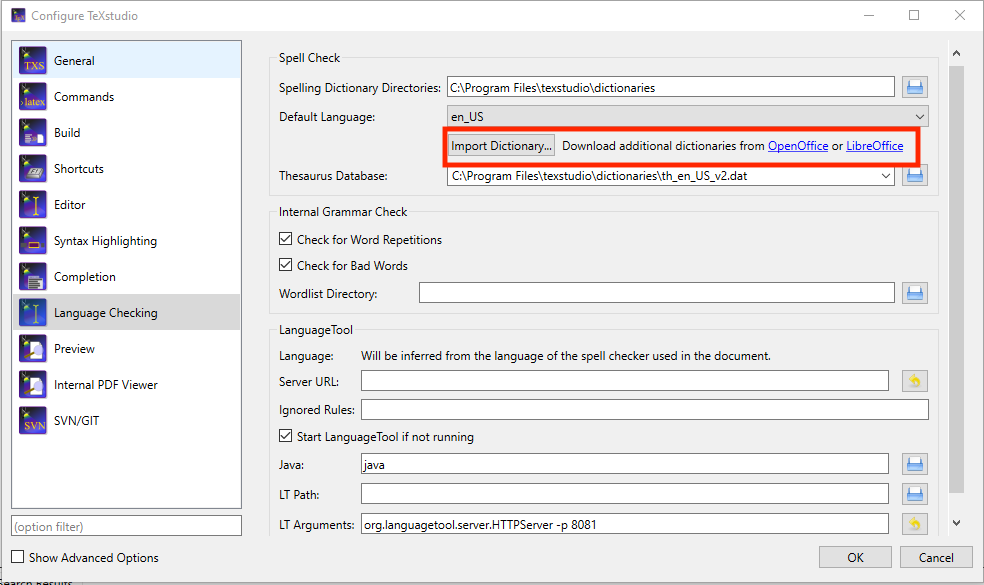
\includegraphics[width=0.8\linewidth]{./lang-check.png}
\end{center}

Texstudio软件会对编译过程中产生的错误和警告会在软件底部的`Message’栏显示给用户。通过双击改错误或警告,光标会自动跳转至相应的位置:如果是\TeX{}文档中的写法错误,光标会自动跳转至出现错误的行;如果是其他错误,如宏包调用问题、字体调用问题,则会跳转至相应的宏包文件。
\begin{figure}[htbp]
     \centering
     \begin{minipage}[c]{0.45\linewidth}
          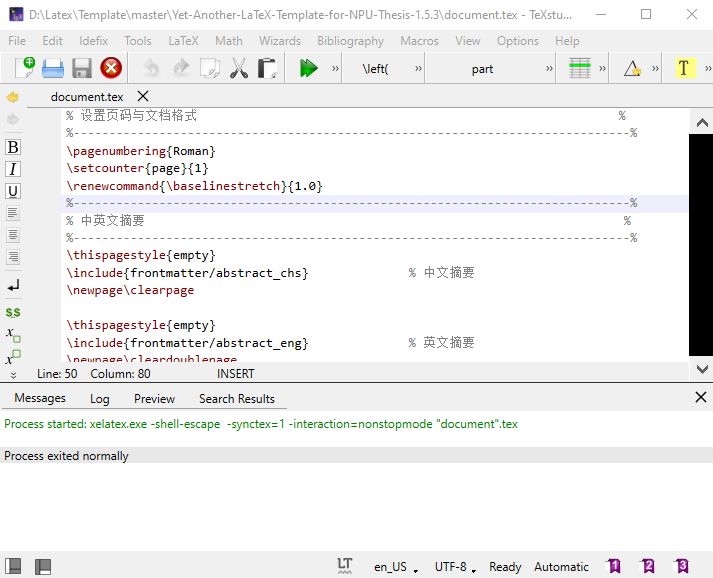
\includegraphics[scale=0.4]{texstudio-message.png}
     \end{minipage}
     \begin{minipage}[c]{0.4\linewidth}
          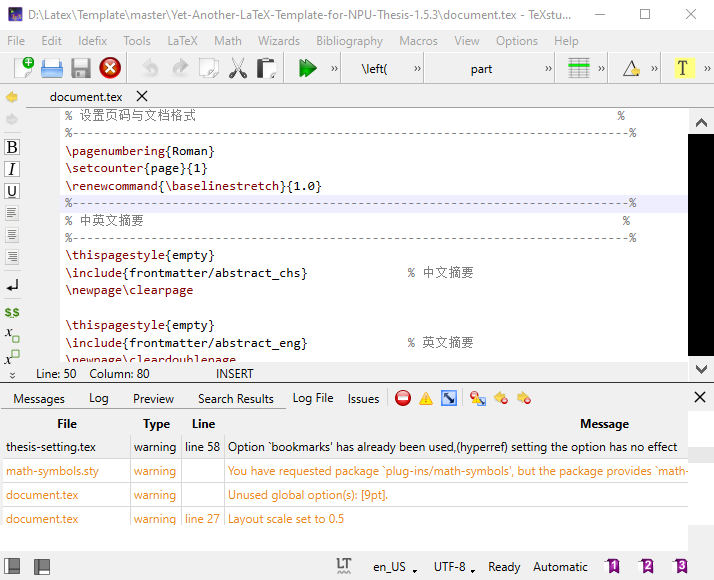
\includegraphics[scale=0.4]{texstudio-error.png}
     \end{minipage}
     \caption{Message信息栏}
\end{figure}



\subsection{Texwork}

\subsection{Texmaker}

\subsection{Vim和sublime}
(Texworks、Texstudio、Texmaker、Vim、其他)配置

\chapter{宏包介绍}

\section{常用宏包}

\LaTeX{}中常用的宏包可以分为几个大类:整体环境设置、图形类、表格类、公式类,此处仅介绍使用率较高的一些宏包。



\section{格式设置类宏包}


ctex:中文\LaTeX{}文档框架,默认包含了ctexart、ctexrep、ctexbook三种不同的文档类型。对与中文使用者来说可以免去较多的格式设定问题。\\
geometry:用于设定输出文章的纸张大小、页边距等尺寸相关的内容。\\
layout:用于对文章内容的页面布局,横版、竖版等布局进行设定。\\
fancyhdr:用来自定义页眉、页脚的内容、格式。\\
afterpage:用来处理图表在页面的浮动。\textit{float和afterpage的区别是啥?}\\
multicol:提供了全文和局部分栏处理功能。但该功能会影响浮动体(图表)的处理,建议在分栏环境内不使用浮动体,例如图、表格等。\\
titlesec:用来对文档内容的标题格式进行设定。一级标题、二级标题等的字体、大小、位置、颜色等进行设定。\\
titlesoc:用于对整个文档的目录格式管理。\\
hyperref:给文档的内容提供一个超文本的链接功能。\\
minted:用于提供格式话的代码引用环境,包含了大量的编程语言以及非编程语言。同时需要配合Pygments(Python)软件包以及`-shell-escap' 编译参数。


\section{字体类宏包}

\noindent xeCJK:提供中文字体设置 \\
fontspec:提供西文字体的自定义设置

\section{插图类宏包}

\noindent graphicx:用于文档内容的插图处理,插图位置、插图大小(比例缩放、非比例缩放)、插图类型以及多行图片的环境。\\
subfigure:用于多子图及子图标题的设置。\\
wrapfig:用于特殊情况的插图设定,例如文字环绕、半环绕等情形。\\
caption:用于对文档中的插图标题进行自定义格式设定,字体、位置、大小等。\\
sidecap:用于一些特殊情形的图题设定,例如外文文档的侧边图题设定。 \\
metalogo:提供\LaTeX{} Logo。

\section{表格类宏包}


\noindent array、table:提供普通的表格设置功能。\\
longtable:提供了跨页表格功能。\\
tabularx:提供了表格内嵌套高级功能的功能。\\
dcolumn:表格内多位小数的对其功能,从小数点对齐。\\
multirow:单元格合并功能。\\
makecell:单元格内设置单元格。\\
diagbox:左上角表头内斜线表格。\\
booktabs:三线表。 \\
rotfloat:旋转表格

\section{公式类宏包}


\noindent amsmath:提供数学公式的编辑环境,如行间公式和行内公式等。\\
ppchtex:提供化学符号。\\
harpoon:提供上下带箭头的字符。

\section{参考/注释类宏包}

\noindent bibtex:文献类型。\\
natbib:文献引用显示类型。\\
footbib:脚注式引用。\\
gbt7714:显示中文文献格式。\\
gloss:附录中的注释表。\\
listings:插入代码。

\chapter{文档类型}

\section{文档类型}

\LaTeX{}中的文档类型(documentclass)可以分为:期刊、报告、书籍、幻灯片(beamer)、书信等。

\subsection{期刊}

\subsubsection{中文双列}
在期刊类型的排版的文档,为了节省版面,经常需要安排双列排版。在documentclass中设定相关选取为:twocolumn即可实现双列排版。但文章标题和摘要(中英文)却又是单列排版,要想实现这种排版,在导言区之后,采用如下代码结构,即可实现标题和中英的单列排版。

\begin{minted}[breaklines]{tex}
    \twocolumn[
    \begin{@twocolumnfalse} % let the two column mode fail temporary。
        \maketitle % maketitle command must put in this environment.
        \begin{document} % after this, abstract and main session start.
        \begin{abstract}
            \textbf{Abstract}:
            \noident Keywords:
        \end{abstract}
    \end{@twocolumnfalse}]     
\end{minted}
    
该模式下,占据单列位置的图片可以在h参数的作用下,在插入图片的位置显示;而双列的图片和表格的位置则很难,会被默认放在页面的底部或顶部。
    
\section{文档结构}


Book类型的文章结构:

$\backslash$part,$\backslash$chapter,$\backslash$section,$\backslash$subsection,$\backslash$subsubsection。一般用来排版较大的学术出版物(或学位论文)。

Arctile类型的文章结构:

$\backslash$part,$\backslash$section,$\backslash$subsection,$\backslash$subsubsection, 以及Abstract。一般用来排版会议、期刊稿件等文档。

Report类型的文章结构:

$\backslash$part,$\backslash$chapter,$\backslash$section,$\backslash$subsection,$\backslash$subsubsection, Abstract 单独成页且包含页码。

\section{目录及章节编号}
    
\subsection{目录编号}
    
目录在不同的文章类型中的要求不尽相同,学术文章中很少用的目录,而学位论文的排版中则需要出现目录,而且列表和插图也要体现在目录中,因此目录进行深度控制。在\LaTeX{}中采用$\backslash$setcounter\{tocdepth\}\{X\}命来来实现不同深度的目录。$\backslash$setcounter\{secnu-mberdepth\}\{Y\} 来实现章节编号的深度。
    
    \begin{center}
        \begin{itemize}
            \item -1 part                    
            \item  0 chapter               
            \item  1 section                
            \item  2 subsection          
            \item  3 subsubsection     
            \item  4 paragraph            
            \item  5 subparagarph   
        \end{itemize}
    \end{center}
    
    
利用$\backslash$renewcommand命令,将文档的一些标题从英文转化为中文标题。如:$\backslash$renew command$\backslash$abstractname\{$\backslash$hei 摘要\},将英文abstractname改为摘要。
    
%\begin{minted}% breaklines,用于自动换行;columns空格控制,fixed默认参数,flexible灵活处理空格,fullflexible强制使用空格。
%\renewcommand\abstractname{\hei 摘要}
%\renewcommand\refname{\hei 参考文献}
%\renewcommand\figurename{\hei 图}
%\renewcommand\tablename{\hei 表}
%
%\newtheorem{dingyi}{\hei 定义~}[section]
%\newtheorem{dingli}{\hei 定理~}[section]
%\newtheorem{yinli} [dingli]{\hei 引理~}
%\newtheorem{tuilun} [dingli]{\hei  推论~}
%\newtheorem{mingti}[dingli]{\hei 命题~}
%\newtheorem{lizi}{<!-- -->{例子}}
%\end{minted}

\subsection{章节编号}

\LaTeX{} 默认的章节编号大多是以阿拉伯数字开始的,但是对于一些经常采用非阿拉伯数字编号的使用者来说就显得有点不友好。因此,在进行章节编号的时候,使用者就需要根据自己的需要来对章节的编号进行自定义。\LaTeX{}中的提供了几类编号方式:$\backslash$arabic 阿拉伯数字,$\backslash$roman 小写的罗马数字,$\backslash$Roman 大写的罗马数字,$\backslash$alph 小写字母,$\backslash$Alph 大写字母。如果使用者希望采用非阿拉伯数字的方式进行编号,利用$\backslash$renewcommand命令进行定义编号的格式。在整理液压传动的时候对章节的编号进行自定义的代码如下:

\begin{minted}[breaklines]{tex}
    \renewcommand{\thesection}{\color[RGB]{60,113,183} \arabic{chapter}-\arabic{section}} %设置section的格式为章序号-节序号
    \renewcommand{\thesubsection}{\chinese{subsection}、} %子节的序号为中文序号+顿号
    \renewcommand{\thesubsubsection}{\arabic{subsubsection}.} 
\end{minted}

\chapter{字体处理}



\section{文字格式}

\subsection{字体}

在\LaTeX{}中要使用自定义的字体,先在导言区调用字体宏包$\backslash$usepackage\{fontspec\},然后用三个命令来设置主字体族、无衬线字体族和打字机字体族$\backslash$setmainfont\{fontName\}, $\backslash$setsansfont\{fontName\}, $\backslash$setmonofont\{fontName\}。当然也可以根据自己的需要对三种字体进行自定义设置,

%$\backslash$setmainfont[BoldFont=boldFontName,ItlicFont=italicFontName]\{mainFontName\}。

在正文中采用$\backslash$textrm\{\}和$\backslash$rmfamily,$\backslash$textsf\{\}和$\backslash$sffamily,$\backslash$texttt\{\}和$\backslash$ttfamily来调用主字体族、无衬线字体族和打字机字体族。两类命令的区别在于前者是将参数(大括号内的部分)变成对应的字体族,而后者是将该命令作用的区域范围内的文字秉承对应的字体族。例如:
\{$\backslash$rmfamily This is rmfamily and $\backslash$textrm\{this is textrm\}\}, this is the main font.

那么排版出来的结果是

{\rmfamily This is a rmfamily and \textrm{This is textrm}}, this is a the main font. %Font is not set, so the difference is not clearly.


使用$\backslash$textup\{\}和$\backslash$upshape, $\backslash$textit\{\}和$\backslash$itshape来分别主动调用当前字体族的直立体与意大利斜体,用$\backslash$textmd\{\}和$\backslash$mdseries, $\backslash$textbf\{\}和$\backslash$bfseries来分别调用当前字体形状的正常体与粗体。

如果想调用第四种低体,可以采用$\backslash$newfonfamily$\backslash$newfontname\{FontName\}来自定义新字体族,FontName为新字体名称;在正文中采用\{$\backslash$newfontname This is a new font\}。

\subsection{字体大小}

\LaTeX{}中字体的大小取决于定义文档类型时设定的字体大小,又被称为绝对字体大小。表\ref{absolute-font}列出了标准文档中的字体绝对大小,单位为pt。例如:
\begin{minted}{tex}
  \documentclass[a4,12pt]{article} 
\end{minted}
此处定义了一个期刊文章类型的文档,采用A4纸张大小,绝对字体大小12pt。如在文章中采用\textbackslash tiny字体,则字体的大小会被认为是6pt,参见表\ref{absolute-font}。其他的字体大小可按照类似的方法设定。但在实际使用过程中也可以根据需要采用\textbackslash fontsize\{<size>\}\{<base line-skip>\}进行任意设定。

\begin{longtable}{|c|m{4.5cm}<{\centering}|m{3.5cm}<{\centering}|m{2.5cm}<{\centering}|}
    \caption{\label{absolute-font}标准文档类中的字号大小。}
    \\
    \hline
    字号 & 10pt & 11pt & 12pt\\
    \hline
    \endfirsthead
    \multicolumn{4}{l}{Continued from previous page} \\
    \hline
    
    字号 & 10pt & 11pt & 12pt \\
    
    \hline
    \endhead
    \hline\multicolumn{4}{r}{Continued on next page} \\
    \endfoot
    \endlastfoot
    \hline
    \textbackslash tiny & 5pt & 6pt & 6pt\\
    \hline
    \textbackslash scriptsize & 7pt & 8pt & 8pt\\
    \hline
    \textbackslash footnotesize & 8pt & 9pt & 10pt\\
    \hline
    \textbackslash small & 9pt & 10pt & 10.95pt\\
    \hline
    \textbackslash normalsize & 10pt & 10.95pt & 12pt\\
    \hline
    \textbackslash large & 12pt & 12pt & 14.4pt\\
    \hline
    \textbackslash Large & 14.4pt & 14.4pt & 17.28pt\\
    \hline
    \textbackslash LARGE & 17.28pt & 17.28pt & 20.74pt\\
    \hline
    \textbackslash huge & 20.74pt & 20.74pt & 24.88pt\\
    \hline
    \textbackslash Huge & 24.88pt & 24.88pt & 24.88pt\\
    \hline
\end{longtable}

\subsection{字体修饰}


在\LaTeX{}中对文字加粗、斜体、强调等操作分别通过以下代码实现:

\begin{minted}{tex}
    %加粗
    \textbf{}% 文本加粗
    \boldmath{} % 数学环境内加粗,需要调用amsmath宏包
    \boldsymbol{} % 可以对希腊字母加粗,需要调用amsmath宏包
    
    %斜体
    \textit{}
    
    %强调
    \emph{}
\end{minted}

特别的,当需要对局部文件进行下划线与其他文字进行区别的时候需要注意,默认的\textbackslash
underline
命令可以实现文字的下划线功能,但是当下划线部分的文字段落过长需要换行的时候,该命令就无法实现了。因此,需要对此进行重点说明。
在\LaTeX{}中英文和中文的下划线换行过程中需要采用不同的宏包进行处理。具体用法如下:
\begin{minted}[breaklines]{tex}
    %下划线
    \underline{} %此命令可以在文字下面生成下划线,但无法在行末进行自动换行。
    
    % 在中文环境中进行换行时采用以下宏包和命令
    \usepackage{CJKfntef} 
    \uline{} 
    
    % 在英文环境中进行换行时采用以下宏包和命令
    \usepackage{ulem}
    \uline
\end{minted}

\subsection{全局字体设置}

\LaTeX{}中的字体可以分为三类:衬线字体(罗马体)、无衬线字体和等宽字体(打字机字体)。

``fontspec"宏包用来设置文档中的西文字体环境。在文档用采用\textbackslash
setmainfont\{\}\textbackslash setsansfont\{\}\textbackslash
setmonofont\{\}三种命令分别来设置西文字体中的衬线体、无衬线体和等宽字体。在使用过程中根据自己的需要采用其中一个命令或多个名来设置相应的字体。

``xeCJK"宏包负责在文档中提供中日韩文字环境。在文档中要显示中日韩文字时,需要\textbackslash
usepackage\{xeCJK\}命令来调用宏包,使用\textbackslash setCJKmainfont
\textbackslash setCJKsansfont\{\}\textbackslash setCJKmonofont\{\}三种命令来设置相应的中文字体。

fontspec和xeCJK的使用方法如下:

\begin{minted}[breaklines]{tex}
    % 拉丁字母设置
    \setmainfont{font name}[font features]%中括号内为字体的特征,如黑体、斜体等。
    \setsansfont{font name}[font features]
    \setmonofant{font name}[font features]
    %中文字体设置
    \setCJKmainfont{font name}[font features]
    \setCJKsansfont{font name}[font features]
    \setCJKmonofont{font name}[font features]
    %举例
    \setCJKmainfont{SimSun}[BoldFont=SimHei,ItalicFont=KaiTi]
\end{minted}

上面的案例中SimHei,KaiTi为操作系统中已经存在的中文字体名称。

关于操作系统中已经存在的中文字体名称的查询方法:
在Windows系统中打开终端程序cmd,输入命令``fc-list :lang=zh"来查询系统中的中文字体,会输出所有中文字体在系统中的相关信息。`fc-list'命令在系统安装texlive之后即可直接使用,但cmd程序中对中文的支持并不友好,此处展示了采用git软件输出的结果,如图\ref{fc-list}。该命令中的字符均为英文状态输入,包括冒号。

\begin{figure}[htbp]
    \centering
    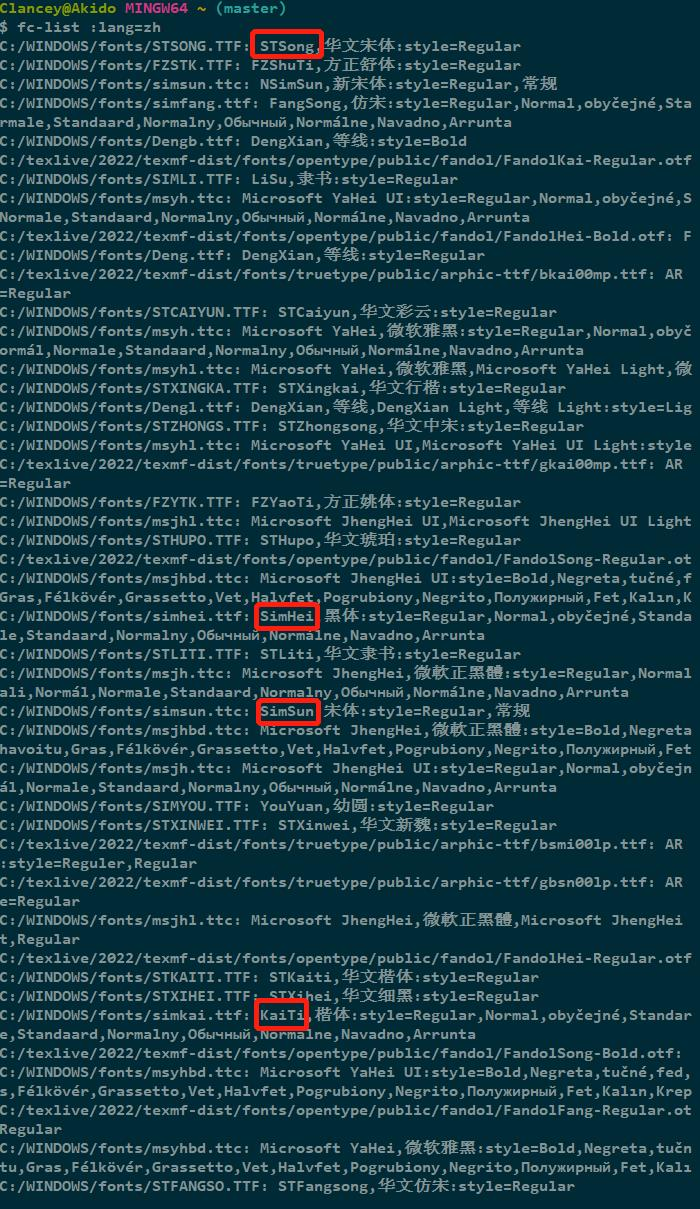
\includegraphics[width=0.8\linewidth]{lang=zh.jpg}
    \caption{fc-list命令结果}
    \label{fc-list}
\end{figure}

图\ref{fc-list}中,红色框位置的内容即为中文字体在系统中的名称,在\LaTeX{}中调用字体,需要输入系统中的字体名称。

在使用ctex宏包时,经常会遇到各种warning,如:

warning 1
\begin{minted}[breaklines]{tex}
    Package fontspec warning: Font "FandolSong-Regular" does not contain
    requested 
    (fontspec)                Script ``CJK"
\end{minted}

warning 2
\begin{minted}[breaklines]{tex}
    Package xeCJK Warning: Redefining CJKfamily `\CJKrmdefault'
    (xeCJK)                (FandolSong-Regular(0))
\end{minted}

warning 3
\begin{minted}[breaklines]{tex}
    Package xeCJK Warning: Redefining CJKfamily `\CJKsfdefault'
    (xeCJK)                (FandolHei-Regular)
\end{minted}

warning 4
\begin{minted}[breaklines]{tex}
    Package xeCJK Warning: Redefining CJKfamily `\CJKttdefault'
    (xeCJK)                (FandolFang-Regular)
\end{minted}

warning1和warning2可以通过对ctex包添加参数来实现。
\begin{minted}{tex}
    \usepackage[fontset=none]{ctex}
\end{minted}

warning2-4可以采用打补丁的方式进行修正。
\begin{minted}{tex}
    \usepackage{ctex}
    \usepackage{xpatch}
\end{minted}

\subsection{局部字体设置}

在\LaTeX{}中如需要对正文中局部字体类型进行自定义,可以通过两类命令来实现:textrm\{\}和rmfamily,textsf\{\}和sffamily,texttt\{\}和ttfamily。这三组命令分别调用衬线字体(罗马体)、无衬线字体、等宽字体(打字机字体)。这两类命令的区别在于:前者是将参数(括号内的部分)设置成对应的字体族,而后者将该命令的作用区域内的文字变成对应的字体族。

\begin{minted}[breaklines=true,breakanywhere,linenos=true]{tex}
    \textrm{This is a example.} % text系列命令对大括号内的字体起作用
    {\rmfamily This is a example.} %family系列命令,需要将自己和需要定义字体的内容都放入大括号内。
\end{minted}

\section{中文字体}

现行的\LaTeX{}版本使用UTF-8作为默认的文字编码。使用拉丁字母的文档保存为UTF-8编码,即可采用pdflatex进行直接编译,但是非拉丁字母,如西里尔字母、希腊字母、阿拉伯字母及东南亚文字等,依然无法直接在\LaTeX{}中直接使用。而较为现代的\TeX{}引擎,如\XeTeX{}和\LuaTeX{},将非拉丁字母文档保存为UTF-8编码,借助fontspec宏包即可实现非拉丁字母的输入。特别的,在使用\LaTeX{}进行中文排版时,需要处理对中文字体的支持,包括:字体设置、行距、断句、标点符号的位置、编译引擎的选择(\XeLaTeX{})等问题。

如果作者在有中文排版需要时,需要在\LaTeX{}中使用中文字体。中文字体的设置方法有两种。第一种采用ctex文档类型,将英文文档的对应类型变为缩写并在前面加ctex。如ctexart,ctexrep等。直接使用命令setCJKmainfont\{fontName\}\}, setCJKsansfont\{fontName\}, setCJKmonofont\{fontName\}来分别设置正文的主中文字体族,无衬线中文字体族和打字机中文字体族。

第二种方法,在tex文档的导言区调用$\backslash$usepackage\{xeCJK\}宏包,然后使用命令setCJKmainfont\{fontName\}, setCJKsansfont\{fontName\}, setCJKmonofont\{fontName\}来分别设置正文的主中文字体族,无衬线中文字体族和打字机中文字体族。但这种方法只定义了字体类型,对中文文章结构并未做优化,如section标题依旧为英文,需要作者自行修改。ctex类文档对中文结构的文档做了优化。

\chapter{格式排版}

\section{段间距}

在不同的段之间,也可以设置段间距(默认为0)。通过$\backslash$setlength\{$\backslash$parskip\}\{parSkip\}来实现。比如说,我想设置段间距为2em, 则使用$\backslash$setlength\{$\backslash$parskip\}\{2em\}即可。这样,在不同两段之间的距离,为段间距+$\backslash$baselineskip的距离。

这里值得注意的是,由于$\backslash$$\backslash$是断行不是分段,所以由$\backslash$$\backslash$引起的下一行与本行之间的距离,只有$\backslash$baselineskip, 而不加上$\backslash$parskip

\section{缩进}

在article及ctexart中,都默认给每一段的段首进行了缩进(在下一篇文章中我们会看到,article中的每一个章节后的首段不会缩进)。我们可以通过$\backslash$setlength\{$\backslash$parinden t\}\{parIndent\}来控制缩进距离,比如说,我想控制段首缩进2em,则应写$\backslash$setlength\{$\backslash$par indent\}\{2em\}. 这个命令会使该命令之后的所有段的缩进都变成这个值。如果要取消全部段落的段首缩进,则可以写$\backslash$setlength\{$\backslash$parindent\}\{0em\}.

如果要单独取消某一行的段首缩进,则在该行的段首写$\backslash$noindent即可。

\section{行距}

因此,在我们改变行距时,如果想把行距调整成精确的值,一般用 $\backslash$fontsize\{fontSize\} \{baseLineSkip\}$\backslash$selectfont来实现;如果想成比例地调整行距,比如单倍行距,双倍行距,则使用$\backslash$linespread\{lineSpread\}$\backslash$selectfont来实现。 比如说,双倍行距就是$\backslash$linespread\{2\} $\backslash$selectfont。

此外,我们也可以用一个名叫setspace的宏包。也就是说,在导言区使用$\backslash$usepackage \{setspace\}.然后使用$\backslash$setstretch\{lineSpread\} 来设置linespread(不用加\selectfont). 这个命令的好处在于会同时修改数学公式、浮动体等的间距,使之与正文间距适应。

\section{自动换行}

\LaTeX{} 中换行的方法针对文字(西文和中文)在操作上略有不同,\LaTeX{}默认对西文进行换行是可以采用$\backslash$ulem package.

对带有下划线的文本进行换行时,如果为英文内容,可采用ulem package提供的$\backslash$uline命令或采用soul package提供的$\backslash$ul 命令来实现。

\section{两端对齐}

两端对齐常用的有两种方法:begin{sloppypar}环境和ragged2e package配合$\backslash$justifying 命令。

\section{页面布局}

在\LaTeX{}中,设置纸张大小的参数是papersize。而papersize的参数如下:a0paper, a1paper, a2paper, a3paper, a4paper, a5paper, a6paper,b0paper, b1paper, b2paper, b3pa per, b4paper, b5paper, b6paper,c0paper, c1paper, c2paper, c3paper, c4paper, c5paper, c6paper,b0j, b1j, b2j, b3j, b4j, b5j, b6j,ansiapaper, ansibpaper, ansicpaper, ansidpaper, ansiepaper,letterpaper, executivepaper, legalpaper 。

自定义页面大小:使用geometry package,结合$\backslash$geometry命令,设置纸张长宽(paperwidth=10cm,paperheight=15cm),页边距(left=0.2cm,right=2.5cm,top=0.5cm,bottom=0.5cm),文字区域的长宽(textwidth=7.3cm)等参数。完整命令如下:

\begin{minted}[breaklines,breakanywhere]{tex}
     \geometry{paperwidth=10cm,paperheight=15cm,left=0.2cm,right=2.5cm,top=0.5cm,bottom=0.5cm,textwidth=7.3cm,textwidth=12cm}
\end{minted}


\section{页眉页脚}

在用 \LaTeX{} 排版文章、书籍时,缺省定义了四种页眉页脚的格式:

\begin{table}[h]
    \centering
    \begin{tabular}{ll}
        empty      & 没有页眉和页脚              \\
        plain      & 没有页眉,页脚中部放置页码        \\
        headings   & 没有页脚,页眉包含章节的标题和页码    \\
        myheadings & 没有页脚,页眉页码和使用者所定义的信息 
    \end{tabular}
\end{table}

对于article 类文档缺省使用 plain 格式,而 book类文档则使用 headings 格式。一般情况下,\LaTeX{}提供的这四种格式基本可以满足大多数的排版需求。但是在某些特殊的情况下,特别是使用者想在某一些页面使用自定义的页眉页脚或全文使用自定义的页眉页脚,这时就会遇到很多限制和麻烦。例如,仅想在某些页面不出现任何页眉页脚,而其余部分按照正常情况还显示页眉页脚,这个时候就可以使用$\backslash$pagestyle命令,其用法为$\backslash$pagestyle\{empty\},将其放置在需要取消页眉页脚的部分,变可实现取消页眉页脚的作用。用法如下:
\begin{minted}[breaklines]{tex}
    %\input{preface}   %引言部分
    \newpage  %原文档为双面,故此处插入空白页面
    \thispagestyle{empty}  %清除引言部分的页眉页脚信息
\end{minted}
\begin{minted}[breaklines]{tex}
    \usepackage{cite}
    
    这里是正文\cite{bib2,bibt2,bibt3}
\end{minted}

但对于那些完全需要自定义页眉页脚的格式的使用者来说,还需要使用额外的宏包"fancyhdr"。该宏包的主要通过定义$\backslash$fancyhead和$\backslash$fancyfoot两个命令对页眉页脚进行控制,这两个命令的参数如下。在编辑教材的时候,由于书籍采用了双面显示,奇数页的页眉不同且没有页脚的显示方式,故利用"fancyhdr"对页眉页脚进行了重新定义。使用的代码如下。
\begin{table}[h]
    \centering
    \begin{tabular}{ll}
        E &     偶数页\\
        O &     奇数页 \\
        L &     页眉或页脚的左边部分\\
        C &     页眉或页脚的中间部分\\
        R &     页眉或页脚的右边部分\\
        H &     页眉\\
        F &     页脚
    \end{tabular}
\end{table}
\begin{minted}[breaklines]{tex}
    \requirepackage{fancyhdr}
    \fancyhf{} 
    %fancyfoot[c]{\color{structurecolor}\scriptsize\thepage} %取消页脚页码
    \if@twoside
    \fancyhead[CO]{\color{structurecolor}\cnormal\leftmark} %leftmark章节名称,奇数页页眉中部显示章节名称
    \fancyhead[OR]{\color{structurecolor}\cnormal\thepage} %奇数页右侧页码
    \fancyhead[EL]{\color{structurecolor}\cnormal\thepage} %偶数页左侧页码
    \fancyhead[CE]{\color{structurecolor}\cnormal\@title} % @title教材名称,偶数页页眉中部显示教材名称
    \else
    \fancyhead[R]{\color{structurecolor}\cnormal\rightmark}
    \fi
\end{minted}



\chapter{图表处理}

\section{图形}




\subsection{常规的图片插入方法}

通常在\LaTeX{}中,通常使用的图片都是jpg和png格式。前者存储更小,但质量有损失;而后者可以做到无损压缩。但是这二者都不能做到放大不失真。为了达到放大不失真的效果,就需要采用矢量图。目前的矢量图的格式有:svg,eps,pdf。

在\LaTeX{}中标准插图方法为:
\begin{figure}[htbp]
     \begin{minipage}{0.45\textwidth}
          \begin{minted}[breaklines,breakanywhere]{tex}
           \begin{figure}[htbp]
            \centering
            \includegraphics[scale=0.5]{filename.png}
            \caption{name of figure}
            \end{figure}
          \end{minted}
     \end{minipage}
     \begin{minipage}{0.45\textwidth}
          \centering
          
\includegraphics[scale=0.2]{logo.png}
          \caption{name of figure}
     \end{minipage}
\end{figure}

\textbackslash includegraphics命令支持的图片格式为jpg,png,eps,pdf。不支持svg格式的矢量图。如果要插入svg格式的矢量图,则需要采用svg宏包。使用方法如下:

\begin{figure}[htbp]
     \begin{minipage}{0.45\textwidth}
          \begin{minted}[breaklines,breakanywhere]{tex}
           \usepackage{svg}
           \begin{figure}
           \centering
           \includesvg{filename.svg}
           \caption{name of svg}
           \end{figure}
          \end{minted}
     \end{minipage}
     \begin{minipage}{0.45\textwidth}
          \centering
          %\includeinkscape[inkscapeformat=pdf,scale=0.3]{logo-svg.svg}
          \includesvg[scale=0.3]{logo-svg.svg}
          \caption{name of svg}
     \end{minipage}
\end{figure}


如果在使用svg格式的矢量图时,出现字体和大小不正常现实的时候,采用\textbackslash usepackage [inkscapelatex=false]\{svg\}。

插入图片的时候,可以给\textbackslash includegraphics命令加上option选项,可以实现比例和长宽的自定义。
\begin{figure}[htbp]
     \begin{minipage}{0.45\textwidth}
          \begin{minted}[breaklines,breakanywhere]{tex}
          \begin{figure}
          \centering
          \includegraphics[width=5cm]{finename.png}
          \caption{name of figure}
          \end{figure}
          \end{minted}
     \end{minipage}
     \begin{minipage}{0.45\textwidth}
          \centering
          
\includegraphics[width=3cm]{logo.png}
          \caption{name of figure}
     \end{minipage}
\end{figure}

\textbackslash caption命令在\textbackslash includegrpahics 的前后决定了图题在图片的前后位置。

特别的对eps格式的图片,由三种方法进行调用。

第一种,采用psfig宏包。

\begin{minted}[breaklines]{tex}
     \usepackage{psfig}
     \psfig{figure=图片文件名,height=高度} \\
     \psfig{figure=图片文件名,width=宽度}
\end{minted}

第二种,采用epsfig宏包。

\begin{minted}[breaklines]{tex}
     \usepackage{epsfig}
     \epsfig{figure=图片文件名,height=高度} \\ %或者
     \epsfig{figure=图片文件名,width=宽度}
\end{minted}


第三种,采用epsf宏包。

\begin{minted}[breaklines]{tex}
     \usepackage{epsf}
     \epsfxsize=宽度\epsffile{图片文件名} \\ %或者
     \epsfysize=高度\epsffile{图片文件名}
\end{minted}

其中的"高度"和"宽度"是指希望图片打印的高度和宽度, 必须给出单位, 可用厘米(cm)或英寸(in)。

\subsection{调用法插入图片}


在\LaTeX{}文章排版过程中,会遇到一种情形:希望引用文献中的图片,但是无法找到文献中的图片原文件,采用截图的方式可能会使图片的清晰程度下降。可以利用includegraphics的不同参数选项来实现。举例如下:
\begin{minted}[breaklines]{tex}
     \usepacage{graphicx}
     
     \begin{figure}
          \centering
          \includegraphics[page=xx,viewport=xx yy zz nn,clip,scale=rate]{./filename.pdf}
     \end{figure}
\end{minted}

includegraphics的选项中,page表示页码,viewport表示希望引用的图的位置,用xx yy表示图片的左下角的坐标值,zz nn表示图片的右上角的坐标值,scale用来设置缩放比例。在\LaTeX{}中,默认纸张的左下角为坐标原点。filename.pdf即含有希望引用图片的原文件。

\subsection{图片位置的排版}


1.浮动

在\LaTeX{}中,图片的位置通常会遵循浮动的原则。在figure环境添加浮动选项可以控制图片的浮动位置。

figure的参数中,h表示当前位置,t表示顶部,b表示底部,p表示浮动。通常遵循h-t-b的顺序。单用h参数是没有效果,常用的选项ht,htbp。如果强制需要图片在某个位置不变,可以采用float宏包,提供的[H]选项。但出现的空白页情况,则需要手动调节。

2.环绕

对一些特殊的期刊文章,需要在文章的开始地方有问题环绕图片的情形。此时需要wrapfig宏包提供的wrapfigure环境来实现。wrapfigure的参数:[number]\{r\}\{0.5$\backslash$textwidth\}行数,位置,宽度

\begin{minted}[breaklines,breakanywhere]{tex}
     \usepackage{wrapfig}
     \begin{wrapfigure}[number]{r}{0.5\textwidth}
          \centering
          \includegraphics[scale=0.8]{filename}
          \caption{title of fig}
\end{minted}

3.子图

在文章排版过程中遇到需要多图并列的效果,需要由subfigure宏包提供的子图环境来实现。

\begin{minted}[breaklines]{tex}
\usepackage{graphicx}
\usepackage{folat}
\usepackage{subfigure}
     \begin{document}
          \begin{figure}[H]
               \centering  %图片全局居中
               \subfigure[name1]{
               \label{Fig.sub.1}
               \includegraphics[width=0.45\textwidth]{filename1}}
               \subfigure[name2]{
               \label{Fig.sub.2}
               \includegraphics[width=0.45\textwidth]{filename2}}
               \caption{Main name}
          \end{figure}
     \end{document}
\end{minted}
4.(多行)并列

学术文献中经常会让多张结果照片并列显示,有时可能还会出现多行并列显示。这个功能可以通过minipage环境来实现。
\begin{minted}{tex}
     \begin{figure}[htbp]
         \begin{minipage}{0.45\linewidth}
          \centering
               \includegraphics[scale=0.15]{filename1.png}
          \end{minipage}
          \begin{minipage}[c]{0.45\linewidth}
               \includegraphics[scale=0.15]{filename2.png}
          \end{minipage}
          \caption{name of figure}
     \end{figure}
\end{minted}

5.图题设置

\LaTeX{}默认的图题中含有冒号,根据需要将冒号去掉或改成点。
\begin{minted}[breaklines]{tex}
     \usepackage{caption}
     \captionsetup[figure]{label=period} %period 表示图xx和标题之间有符号``点"。
     \captionsetup[table]{label=space} %space 表示图xx和标题之间为空格。
\end{minted}

在排版过程遇到图片或图题距离上下的距离或图片和图题之间的距离需要调整的情形,可以采用一下代码。
\begin{minted}[breaklines]{tex}
     \vspace{-1cm} %调整图片与上文的垂直距离
     \setlength{\abovecaptionskip}{-0.5cm} %调整图片标题与图距的距离
     \setlength{\belowcaptionskip}{-0.5cm} %调整图片标题与下文之间距离
\end{minted}

\subsection{图片引用}

在文章中对图片进行交叉引用方法如下:

\begin{minted}[breaklines]{tex}
     \usepackage{graphicx}
     \usepackage{float} 
     \usepackage{subfigure}
     \usepackage{caption}
     \begin{document}
          \begin{figure}[H]
          \centering  %图片全局居中
          \subfigure[name1]{
               \label{Fig.sub.1}
               \includegraphics[width=0.45\textwidth]{filename1}}
               \subfigure[name2]{
                    \label{Fig.sub.2}
                    \includegraphics[width=0.45\textwidth]{filename2}}
               \caption{Main name}
               \label{Fig.main}
          \end{figure}
\end{minted}


\subsection{图形编号}

\LaTeX{}在处理图形编号时,会自动根据$\backslash$begin\{figure\}和$\backslash$end\{figure\}对图形的编号进行自动累加。在实际使用过程中,会经常遇到一些好几个图公用一个图题的情况,如果将这些图都放置在一个环境中,有些图可能会因为纸面大小的关系而无法显示,但是如果分开放置到两个或三个图形环境中,这些图题会自动增加。此时需要使用$\backslash$ContinuedFloat命令,即可让图的编号不自动增加,而是和上一个环境链接起来,当一个图形环境来使用。在液压传动教材中的多图排版中采用如下的方式让图形编号不间断。
\begin{minted}[breaklines]{tex}
    \begin{figure}[htbp]
         content...
    \end{figure}
    \begin{figure}[htbp]
         \ContinuedFloat %链接上下两个图形环境,使其编号不自动增加
    \end{figure}
\end{minted}

一般的图形标题都比较短,所以在显示的过程中不会出现比较一些换行的问题。但是对于一些比较长的图题,而且图处于文字环绕的环境中,图题的换行问题就显得比较突出和重要了。图题的换行问题可以利用宏包``caption"配以相应的参数hang即可解决。caption产生的图题中的图号和文字之间产生一个冒号,通过$\backslash$captionsetup的参数labelsep=space即可去除这个冒号。
\begin{minted}[breaklines]{tex}
     \requirepackage[font=small,labelfont={bf,color=sturcturcolor},hang]{caption} %hang解决了图题过长时的自动换行问题
     \captionsetup[table]{skip=3pt}
     \captionsetup[figure]{skip=3pt}
     \captionsetup{labelformat=default,labelsep=space} %去除图片编号中的冒号
\end{minted}

去除图表caption中的冒号。
\begin{minted}[breaklines]{tex}
     \usepackage{caption}
     \captionsetup[table]{labelsep=space} % 表
     \captionsetup[figure]{labelsep=space} % 图
     
     \captionsetup{labelformat=default,labelsep=space} %去除冒号
\end{minted}
  


\subsection{图形的浮动和环绕}

通常我们在 \LaTeX{} 插入图片时,要为图片单独设置一个环境,即$\backslash$begin\{figure\}和$\backslash$end\{figure\}。
\begin{minted}[breaklines]{tex}
     \begin{figure}
          \includegraphics[keyvals]{imagefile}
     \end{figure}
\end{minted}

在这个环境中可以设置输入图片的类型,$\backslash$includegraphics命令来实现对输入图片的操作。常用的一些基本参数如下:

\begin{table}[h]
     \centering
     \begin{tabular}{ll}
          height &     图形的高度(可为任何 TEX 度量单位)。\\
          totalheight     & 图形的全部高度,可为任何 TEX 度量单位( 6/95 增加)。\\
          width &     图形的宽度(可为任何 TEX 度量单位)。\\
          scale     & 图形的缩放因子,设定 scale=2 会使 插入的图形的大小为其自然大小的两倍。\\
          angle &     设定旋转的角度,以度为单位,顺时钟方向为正。\\
     \end{tabular}
\end{table}

对于经常使用\LaTeX{}进行论文排版的使用者来说,常见的图片排版问题莫过于多图的并列排版。对于实现多图排版,\LaTeX{}中要多种方式可以实现。当图片的版幅较大,无法两图并排放在一起,如果缩放不影响显示效果的情况下,可以连用$\backslash$includegraphics来实现,并列排放的效果。另外也可以利用$\backslash$minipage环境来实现多图的并列。

\begin{minted}[breaklines]{tex}
     \begin{figure}[htbp] % htbp用来浮动,h-here,t-top,b-buttom
          \centering
          \includegraphics[scale=0.9]{fig0203.pdf}
          \includegraphics[scale=0.9]{fig0204.pdf}
     \end{figure}
\end{minted}

\begin{minted}[breaklines]{tex}
     \begin{minipage}[t]{0.48\textwidth} %设置图形宽度
          \centering
          \includegraphics{fig0124.pdf}  
     \end{minipage}
     \begin{minipage}[t]{0.48\textwidth}
          \centering
          \includegraphics{fig0125.pdf}  
     \end{minipage}
\end{minted}

在对图片进行排版的过程中,可能会遇到图片较小或图片宽度较小、长度方向较大的情况,如果此时对图片进行单独占行进行排版,会留下大量的空白,影响整体的排版的美观性。因此,在排版过程中对图片进行环绕处理。在对图片的环绕处理时利用的$\backslash$begin\{wrapfigure\}和$\backslash$end\{wrapfigure\}环境来实现。wrapfigure的参数主要分为:[行数]、\{位置\}、\{宽度\}。

\begin{minted}[breaklines]{tex}
     \begin{wrapfigure}[num]{r}{8cm}% num表示要环绕的行数,r和l分别表示从右侧和左侧环绕;8cm为环绕留给图形的宽度
          \centering
          \ifOpenSource
          
\includegraphics[width=5cm]{logo.png}
          \else
          \includegraphics{fig0201.pdf}
          \fi
          \caption{能量转换示意}
          \label{fig:fig0201}
     \end{wrapfigure}
\end{minted}


对于一些占幅面较大的图片,可能需要横向排布才能显示较全的信息,此时有两种方式来实现图片的旋转功能。$\backslash$includegraphics[angle=xxx]\{fig.png\}或利用$\backslash$begin\{side waysfigure\}和$\backslash$end\{sidewaysfigure\}来实现。
\begin{minted}[breaklines]{tex}
     \begin{figure}[htbp]
          \centering
          \includegraphics[angle=xxx]{imagefile} %图片旋转,可自定义旋转角度
          \caption{text}
     \end{figure}
\end{minted}

\begin{minted}[breaklines]{tex}
     \begin{sidewaysfigure} %图片横向排版环境
          \centering 
          \includegraphics[width=4in]{graphic.eps} 
          \caption{Sidewaysfigure Figure} 
     \end{sidewaysfigure}
\end{minted}

通常情况下,图片和文字是按照一定顺序来进行排放的。但是有些期刊的排版会要求作者将图片和文字分开排版,即文字在前,图片和表格在后的排版方式。在\LaTeX{}中实现这种文字在前、图片在后的排版方式,仅需引入一个endfloat宏包即可实现。

\begin{minted}[breaklines]{tex}
     \usepackage[noheads,nolists,nomarkers]{endfloat}
     \renewcommand{\efloatseparator}{\mbox{}}
\end{}

\section{表}

\chapter{公式}

\section{常用公式录入}


\LaTeX{}中数学公式的排版,大部分功能都由amsmath宏包提供。amsfont、amssymb宏包提供了大量的数学符号;amsthm宏包提供了扩展的\LaTeX{}定理证明格式。


\subsection{行内公式}


行内公式,顾名思义,公式在文字的行内,属于文字公式混排。此类公式没有公式编号,通常由一对``\$"包裹,例如:

\begin{example}
勾股定理可表示为:$a^{2}+b^{2}=c^{2}$。
\end{example}

\subsection{行间公式}


行间公式处于文字段落之外,可以采用equation环境书写,此时行间公式默认有公式编号。采用equation*环境可以提供不带编号的行间公式。利用\textbackslash
ref命令来进行引用,或利用amsmath宏包提供的\eqref(会默认对引用添加括号)命令来进行引用。如果需要自定以公式编号,可以采用\textbackslash
label进行自定义;也可以采用\textbackslash
tag对公式进行自定义编号;或者采用\textbackslash notag取消公式编号。
\begin{example}
\begin{equation}
    a^{2} + b^{2} = c^{2} \label{Pythagoras}
\end{equation}
公式\eqref{Pythagoras}被称为勾股定理。
\end{example}

如果需要不提供编号的行间公式,可以采用\textbackslash[和\textbackslash]提供的行间公式环境或者利用displaymath环境提供的行间公式。
\begin{example}
     \[ a^{2} + b^{2} = c^{2} \]
     
     \begin{displaymath}
          a^{2} + b^{2} = c^{2}
     \end{displaymath}
     
     \begin{equation*}
          a^{2} + b^{2} = c^{2}
     \end{equation*}
\end{example}

\subsection{行间多行公式}


在数学证明方面,可能会出现很长的、需要折行的公式,通过amsmath宏包提供的multline环境来完成。
\begin{example}
  \begin{multline}
     a + b + c + d = e + f + g + h \\
     = i + j + k + l\\
     = m + n + o + p\\
     = q + r + s = t
  \end{multline}
\end{example}

在证明过程中可能会用到多个公式联立,并在等号处对其。此时,可以采用align环境。

\begin{example}
     \begin{align}
          x + y &= 5 \\
          3x + y &= 8
     \end{align}
\end{example}


如果不需要多行公式对其时,则可以采用gather环境完成。
\begin{example}
     \begin{gather}
          x +y = 5\\ %\\用来分割各行
          2x + y = 8
     \end{gather}
\end{example}

multline、gather和align环境都会自动生成公式符号,如果不需要公式编号的时候,在gather和align后面添加“*”,即multline*、gather*和align*。需要注意的是,aligh和gather环境会给每一个公式添加编号;如果只需要一个公式编号,则需要将align或gather嵌套如equation环境中即可。

\subsection{单侧括号公式块}

\begin{example}
	\begin{equation}
		 \left. 
		\begin{aligned}
			x + y & > 10 \\
			x - y  & > 2
		\end{aligned}
		\right \} \Rightarrow x^{2}-y^{2} > 20
	\end{equation}
\end{example}

对一个分段函数来说
\begin{example}
     \[ |x| = \left\{
     \begin{array}{rl}
          -x & \text{if } x < 0,\\
          0 & \text{if } x = 0,\\
          x & \text{if } x > 0.
     \end{array} \right. \]
\end{example}

也可以采用amsmath宏包提供的case环境来实现。

\begin{example}
 \[ |x| =
    \begin{cases}
          -x & \text{if } x < 0,\\
          0 & \text{if } x = 0,\\
          x & \text{if } x > 0.
     \end{cases} \] 
\end{example}



\chapter{参考文献}

\section{参考文献引用}


\LaTeX{}中管理参考文献的方法有两类:一、针对文献数量较少时,可以直接采用thebibliography环境来管理参考文献;二、采用bib文档,调用相应的参考文献格式来进行管理文献。

\subsection{thebibliography}


thebibliography方法相对简单,直接将参考文献的内容存放的document环境之内,清晰明了。当参考文献的数量相对较少,或对参考文献的格式没有特殊的要求时,相对来说是一种比较方便的引用方法。
\begin{minted}[breaklines,breakanywhere]{tex}
     \documentclass{article}
     
     \begin{document}
          
          \section{Introduction}
          
          这是一个测试案例,用来介绍引用参考文献的引用方法\cite{ref1}。\\%ref1只是一个引用符号,可以是任何字符。
          
          \begin{thebibliography}{99}%99是指参考文献的最大数量,可以自行设定
               \bibitem{ref1} xxxxxxxxxxx %和前面的ref1对应,后面添加参考文献的内容。
               \bibitem{ref2} xxxxxxx
          \end{thebibliography}
     \end{document}
\end{}


\subsection{bib}

对参考文献的排版有特殊的格式要求、管理的便捷、大量的参考文献条目、希望\TeX{}文档整体有条理时,可以采用bib文件的方式来进行参考文献管理。
\begin{minted}{tex}
     @article{name1,
          title = {标题},
          author = {作者,多个作者用and连接},
          year = {年份},
          journal = {期刊名称},
          volume = {卷},
          pages = {页码},
          abstract = {摘要},
     }
     
     @mastersthesis{name2,  %masterthesis 表示学位论文。
          type = {硕士},
          title = {标题},
          author = {作者},
          year = {年份},
          abstract = {摘要},
          school = {武汉科技大学},
     }
\end{minted}

在\LaTeX{}文档中,需要引用文献的地方插入文献使用$\backslash$cite命令。在文档结束之前的地方插入bib文件名称。

\begin{minted}[breaklines]{tex}
     \documentclass{article}
     
     \begin{document}
          
          \section{Introduction}
          
          xxxxxxxxxxx
          
          \bibliographystyle{style} %style为希望展示的参考文献格式
          \bibliography{reference} %reference为bib文件的名称,
     \end{document}
\end{minted}

\section{文献检索}

文献信息检索通常是指从以任何方式组成的文献信息集合中,查找特点用户在特定时间和条件下所需要信息的方法和过程。在学术论文写作过程中,需要撰写研究领域内的研究进展,就需要通过检索相同或相近领域内的相应文献。而这些文献信息可以被归纳为:图书、期刊、报告、会议、专利、学位论文等类型,而其中以期刊文献占绝大多数。
\subsection{英文文献检索}

英文期刊文献主要通过几大专业文献数据来进行检索,如WOS、PubMed(医学)、ScienceDirect等。WOS提供了大量的标题和摘要检索,几乎涵盖了中英文期刊、会议、专利等方面文献。

\subsection{中文文献检索}

中国知网CNKI全文数据库是国内规模最大的多功能学术期刊全文检索系统,也是国际上最大的动态持续更新的中文期刊全文数据库。同时CNKI还提供国内的专利、学位论文的检索服务。


文献的检索常用有以下三类途径:学术搜索引擎(谷歌学术、必应学术、百度学术等)、专业数据库(WOS、CNKI、PubMed、ProQuest、ScienceDirect等)以及RSS学术文献追踪。

\section{参考文献管理}

参考文献在科技论文写作中占有非常重要的地位,体现了文章成果有前人研究基础上的继承性。一篇文章的参考文献少则10来篇,多则几百篇。当引用文献数量较少时,手工录入不是什么大问题,但几百篇参考文献在文章中的不同位置出现时,引用起来就很费时、费力,而且容易出错,有可能导致引文与文献编号对应错误。再者在文章中通过纯手工方式插入参考文献,调整起来也很难,特别是文献编号要求从头到尾顺序编排时更是如此。在此,介绍几个比较流行的参考文献管理软件。

作为参考文献管理软件,其功能强大,支持自定义特性,即可以自定义EndNote的输出格式、滤件和链接论文件等。但其不足页非常明显:分组管理功能仅支持二级目录,也不支持标签功能;对中文的支持并不友好;且属于商业软件,个人用户不容易取得授权文件。

\subsection{Mendeley}


ScienceDirect出品,免费使用,支持多平台使用(网页、Windows、Linux、Mac、iPhone、iPad),可以与Word、LibreOffice、\LaTeX{}等无缝链接,文献多级目录管理,支持PDF标记功能。其特色为学术社区群组功能,形成学术小组,组内成员共享文献。但其缺点也非常明确:对中文的支持并不友好。

\subsection{NoteExpress}

后来出现了国产软件 NoteExpress,功能差不多,可以管理文献条目、作为 Word 插件可以在文档中方便插入文献、定制输出样式等,而且可针对中、英文献分别定制输出样式,目前流行度很高。以上提到的参考文献管理软件均为商业软件,经常为版本升级而导致原先建立的文献库无法打开,另使用者痛苦万分。

\subsection{Zotero}


开源软件,利用浏览器插件(支持Chrome、Firefox、Safrai等)和客户端可以无缝抓取网页中的多种参考文献(书籍、会议、学术文章、报纸、电视、报告、手稿、杂质等)。Zotero支持无线级的目录分类,即一个目录下可以生成多个子目录;同时支持文献标签功能,可以对位于不同目录下的文献采用相同的标签管理,对大量文献管理的使用者来说较为方便。在多平台方面,支持Windows、Mac、Linux、iOS,同时每个注册账户赠送300MB的网络同步存储空间。且支持采用WebDav来同步文献中的PDF文件。
具有群组文献管理功能,多个用户加入同一个组(group),可以无限制同步文献条目(不同步文献条目下的附件),如需要同步附件,则需要购买官方提供的网络存储空间。中文支持程度较好,且可以使用GB输出中文参考文献。对word的支持程度良好。


\subsection{JabRef}

开源参考文献管理软件,最大的特点就是基于BibTex格式进行文献管理。其数据库本质上为文本文件,透明度高,存储数据结构化。可以采用其他支持bib格式的参考文献管理软件打开,从而实现多平台和不同写作环境下使用同一个参考文献数据库。

\section{文献引用}


\subsection{西文参考文献}


在\LaTeX{}文档中添加参考文献,需要做好几个步骤:准备bib格式的参考文献,在\LaTeX{}文档中调用相应的宏包,编译生成pdf文档。

bib格式的参考文献必须具备的内容:author,title,journal,volume,year,number。举例如下:

\begin{minted}[breaklines,breakanywhere]{tex}
     @article{name1, %name1为正文中需要引用的关键词,即\cite{name1}。
          title = {文章标题},
          author = {作者, 多个作者用 and 连接},
          journal = {期刊名},
          volume = {卷},
          number = {页码},
          pages={},
          year = {年份},
          publisher={出版社}
     }
\end{minted}

在\LaTeX{}文档中,首先在导言区调用cite宏包,在正文区内设置需要显示的参考文献风格类型,设置参考文献bib文件的位置。\LaTeX{}默认提供的参考文献样式有8种:
\begin{minted}[breaklines,breakanywhere]{tex}
     \centering
     plain,按字母的顺序排列,比较次序为作者、年度和标题.
     unsrt,样式同plain,只是按照引用的先后排序.
     alpha,用作者名首字母+年份后两位作标号,以字母顺序排序.
     abbrv,类似plain,将月份全拼改为缩写,更显紧凑.
     ieeetr,国际电气电子工程师协会期刊样式.
     acm,美国计算机学会期刊样式.
     siam,美国工业和应用数学学会期刊样式.
     apalike,美国心理学学会期刊样式.
\end{minted}

完整的引用案例如下:

\begin{minted}[breaklines,breakanywhere]{tex}
     \documentclass{article}
     \usepackage{cite}
     
     \begin{document}
          这是一个参考文献引用方法的举例\cite{key}。
          \bibliographystyle{unsrt} %设置参考文献的显示风格。
          \bibliography{reference} % reference为存放参考文献的bib文件名,该文件默认和tex主文档放在同一个目录下;如果发生了路径变化,则需要提供相对路径。
          
     \end{document}
\end{minted}
参考文献的引用需要在导言区添加相应的宏包,在正文中需要引用参考文献的地方,添加相应的文献。添加单个或多个不连续的文献,方式如下:

\begin{minted}[breaklines,breakanywhere]{tex}
     \usepackage{cite}%导言区添加
     
     文献表明:这个问题可以通过这种方式来解决\cite{bibtex1,bibtex3,bibtex5}。%正文区
\end{minted}

输入结果如下:

\begin{minted}{tex}
     文献表明:这个问题可以通过这种方式来解决[1,3,5]。
\end{minted}

添加多个连续的参考文献,方式如下:

\begin{minted}{tex}
     \usepackage{cite} %导言区
     \usepackage[number,sort&compress]{natbib} %导言区
     文献表明:这个问题可以通过这种方式来解决\cite{key1,key2,key3}
\end{minted}

输出结果如下:
\begin{minted}{tex}
     文献表明:这个问题可以通过这种方式来解决[1-3]。
\end{minted}


\subsection{中文参考文献}


中文参考文献可以遵循GB/T 7714-2015。使用\LaTeX{}对中文学术论文进行排版时,可以按照GB/T 7714-2015来设置参考文献的格式。用法如下:
\begin{minted}[breaklines,breakanywhere]{tex}
     \documentclass{article}
     \usepackage{ctex}%ctex宏包中包含了cite,可以不必单独调用宏包。
     \usepackage{gbt7714}
     
     \begin{document}
          
          充足的睡眠有利用身体健康\cite{key1}
          
          \bibliographstyle{gbt7714-numerical} %利用GB/T 7714-2015宏包来设置参考文献的格式
          \bibliography{ref} %ref代表存放参考文献的bib文件名称。
     \end{document}
\end{minted}

\section{格式}

\LaTeX{}在文档最后编排的参考文献格式被成为`style',调用时采用$\backslash$bibliographystyle{style},$\backslash$bibliography{reference}。

常见的几种格式如下:

plain,按字母的顺序排列,比较次序为作者、年度和标题.  
unsrt,样式同plain,只是按照引用的先后排序.  
alpha,用作者名首字母+年份后两位作标号,以字母顺序排序.  
abbrv,类似plain,将月份全拼改为缩写,更显紧凑.  
ieeetr,国际电气电子工程师协会期刊样式.  
acm,美国计算机学会期刊样式.  
siam,美国工业和应用数学学会期刊样式.  
apalike,美国心理学学会期刊样式.

\section{插入引文}

首先要在导言区调用宏包$\backslash$usepackage\{cite\};在正文中需要引用文献的地方,输入$\backslash$cite\{bibtex1\},编译之后正文引用文献的地方显示[1]。在文中需要输入多个参考文献的地方输入$\backslash$cite\{bibtex1,bibtex3,bibtex5\},其中每个引用文献之间要英文逗号隔开,输出结果为[1,3,5]。如果要输入的参考文献序号是连续的,则需要在导言区调用新的宏包,$\backslash$usepackage[number,sort\&compress]\{natbib\},正文中的参考文献$\backslash$cite\{bibtex1,bibtex2, bibtex3\},输出结果为[1-3]。

有些文档重要求参考文献的引用标志在正文中要体现在右上角,此时要在导言区自定义新命令,$\backslash$newcommand\{$\backslash$upcite\}[1]\{$\backslash$textsuperscript\{$\backslash$textsupercript\{$\backslash$cite\{\#1\}\}\}\},在正文需要参考文献的地方,用$\backslash$upcite命令来插入参考文献,$\backslash$upcite\{bibtex1\}。


在\LaTeX{}{} 中使用中文参考文献,其格式需要参照GB/T 7714-2015来执行,但是在LaTeX{} 本身的支持中却没有该选项。因此,需要通过自定义功能来实现,在github上https://github.com/zepinglee/gbt7714-bibtex-style。


\section{引文文件}

本文仅用于总结近期使用\LaTeX{}整理书籍的一些常用宏包的用法。

\chapter{批注}

\chapter*{\LaTeX{} 使用总结}


\section{常见错误}

\begin{sidewaystable}
     \centering
     \caption{Ambiguous Errors}
     \begin{tabular}{|c|l|l|l|} 
          \hline
          No & \multicolumn{1}{c|}{Class} & \multicolumn{1}{c|}{Error Message}                            & \multicolumn{1}{c|}{Cause of Error}                                                                                          \\ 
          \hline
          1  & e\_des                     & ! \LaTeX{} Error: There's no line here to end                    & Usage of \textbackslash{}\textbackslash{} at the end of a long label in 'description' environment                            \\ 
          \hline
          2  & e\_center                  & ! \LaTeX{} Error: There's no line here to end                    & Usage of \textbackslash{}\textbackslash{} after the heading line in 'center' environment                                     \\ 
          \hline
          3  & e\_foot                    & ! Argument of \textbackslash{}@sect has an extra \}           & Usage of a fragile command 'footnote' within \textbackslash{}section                                                         \\ 
          \hline
          4  & e\_ragged                  & ! Argument of \textbackslash{}@caption has an extra \}        & Usage of \textbackslash{}\textbackslash{} within \textbackslash{}raggedright or \textbackslash{}raggedleft environment       \\ 
          \hline
          5  & e\_and                     & ! Extra alignment tab has been changed to \textbackslash{}cr  & Too many s in a row of a table or array or eqnarray.                                                                         \\ 
          \hline
          6  & e\_cline                   & ! Extra alignment tab has been changed to \textbackslash{}cr  & Reference no non existing column in \textbackslash{}cline                                                                    \\ 
          \hline
          7  & e\_col                     & ! Extra alignment tab has been changed to \textbackslash{}cr. & Usage @ in tabular* environment                                                                                              \\ 
          \hline
          8  & e\_num                     & ~! Missing number treated as zero                             & Usage of non numeric parameter after \textbackslash{}\textbackslash{}                                                        \\ 
          \hline
          9  & e\_asterisk                & Missing * at the end of the line                              & * is not printed when used without brace after \textbackslash{}\textbackslash{}                                              \\ 
          \hline
          10 & e\_pbox\_miss              & ! Missing number, treated as zero.                            & \textbackslash{}parbox[t]\{\} ..Missing argument to parbox                                                                   \\ 
          \hline
          11 & e\_mis\_circle             & ! Missing number, treated as zero.                            & Missing numeric parameter to \textbackslash{}circle                                                                          \\ 
          \hline
          12 & e\_list                    & ! Argument of \textbackslash{}lst@next has an extra \}        & Usage of 1stlisting inside fragile command \textbackslash{}parbox                                                            \\ 
          \hline
          13 & e\_capacity                & ! TeX capacity exceeded, sorry [input stack size=1500]        & Usage of 1stlisting inside fragile command \textbackslash{}parbox                                                            \\ 
          \hline
          14 & e\_runaway                 & Runaway argument?                                             & Generally because of missing braces, e.g \textbackslash{}cline\{1-2 instead of 
          \textbackslash{}cline\{1-2\}           \\ 
          \hline
          15 & e\_verbatim                & Runaway argument?                                             & Usage of verbatim within scope of another command e.g: \textbackslash{}ifthenelse                                            \\ 
          \hline
          16 & e\_undefined               & ! Undefined control sequence                                  & Usage of an unknown command                                                                                                  \\ 
          \hline
          17 & e\_footnote                & ! Undefined control sequence                                  & Usage of \textbackslash{}footnote within \textbackslash{}footnote                                                            \\ 
          \hline
          18 & e\_integral                & ! Missing \{ inserted.                                        & Integral bounds are malformed                                                                                                \\ 
          \hline
          19 & e\_zeta                    & ! Missing \{ inserted.                                        & Extra subscript before integral upper limit term                                                                             \\ 
          \hline
          20 & e\_bezier                  & ! Illegal unit of measure (pt inserted).                      & Missing numeric argument to \textbackslash{}qbezier                                                                          \\ 
          \hline
          21 & e\_too\_bezier             & ! Illegal unit of measure (pt inserted).                      & Too many arguments to \textbackslash{}qbezier                                                                                \\ 
          \hline
          22 & e\_unit                    & ! Illegal unit of measure (pt inserted)                       & \textbackslash{}parbox[t]\{2\} ..Illegal unit of second parameter                                                            \\ 
          \hline
          23 & e\_symfoot                 & ! \LaTeX{} Error: Counter too large.                             & More than 9 footnotes when using symbolic footnotes                                                                          \\ 
          \hline
          24 & e\_large\_count            & ! \LaTeX{} Error: Counter too large.                             & Trying to display a corresponding letter for a counter vallue 26                                                             \\ 
          \hline
          25 & e\_begin                   & ! \LaTeX{} Error: Missing \textbackslash{}begin\{document\}      & Either text has been placed before \textbackslash{}begin\{document\} or 
          \textbackslash{}begin\{document\} is missing  \\ 
          \hline
          26 & e\_margin                  & ! \LaTeX{} Error: Missing \textbackslash{}begin\{document\}.     & Misuse of \textbackslash{}marginsize                                                                                         \\
          \hline
     \end{tabular}
\end{sidewaystable}

%\begin{sidewaystable}
%     \centering
%     \caption{Common Errors}
%%     \begin{tabular}{|l>{0.05\linewidth}|l|l|l|} 
%          
%%          \multicolumn{1}{|>{\centering}{0.05\linewidth}|}{No} & \multicolumn{1}{c|}{Class} & \multicolumn{1}{c|}{Error Message}                                                              & \multicolumn{1}{c|}{Cause of Error}                                                                                                                                         \\ 
%\begin{tabular}{|>{\centering\hspace{0pt}}m{0.05\linewidth}|>{\hspace{0pt}}m{0.1\linewidth}|>{\hspace{0pt}}m{0.3\linewidth}|>{\hspace{0pt}}m{0.4\linewidth}|} 
%     \hline
%     No  & \multicolumn{1}{>{\centering\hspace{0pt}}m{0.1\linewidth}|}{Class} & \multicolumn{1}{>{\centering\hspace{0pt}}m{0.3\linewidth}|}{Error Message} & \multicolumn{1}{>{\centering\arraybackslash\hspace{0pt}}m{0.4\linewidth}|}{Cause of Error}  \\ 
%     \hline
%          1                        & e\_fileEnd                 & ! File ended while scanning use of \textbackslash{}end.                                         & Generally caused because of missing a brace                                                                                                                                 \\ 
%          \hline
%          2                        & e\_end                     & No message only an asterisk, i.e *                                                              & Missing \textbackslash{}end\{document\}                                                                                                                                     \\ 
%          \hline
%          3                        & e\_illegal                 & \LaTeX{} Error: Illegal character in array arg                                                     & Usage of a letter other than r,l and c in tabular environment                                                                                                               \\ 
%          \hline
%          4                        & e\_tab                     & ! Misplaced alignment tab character                                                             & Missing \textbackslash{}begin\{tabular\} while using tabular environment                                                                                                    \\ 
%          \hline
%          5                        & e\_backslash               & ! Missing \textbackslash{}endcsname inserted                                                    & Usage of a backslash in front of the name of an environment, e.g 
%          \textbackslash{}begin\{\textbackslash{}itemize\}                                                    \\ 
%          \hline
%          6                        & e\_delimiter               & ! \LaTeX{} Error: Bad math environment delimiter                                                   & Missing \textbackslash{}right immediately after the array environment                                                                                                       \\ 
%          \hline
%          7                        & e\_right                   & ! Extra \textbackslash{}right                                                                   & \textbackslash{}right has no matching \textbackslash{}left OR \textbackslash{}end\{array\} is missing                                                                       \\ 
%          \hline
%          8                        & e\_package                 & ! \LaTeX{} Error: Can only be used in preamble                                                     & Usage of \textbackslash{}usepackage outside the preamble                                                                                                                    \\ 
%          \hline
%          9                        & e\_math                    & ! Missing \$ inserted                                                                           & Missing a starting or ending \$ in Math mode, e.g m\_e instead of \$m\_e\$                                                                                                  \\ 
%          \hline
%          10                       & e\_parameter               & ! Illegal parameter number in definition of...                                                  & Usage of parameter number greater than the number of parameters  defined in \textbackslash{}newcommand, e.g \textbackslash{}newcommand\{\textbackslash{}test\}{[}1]\{\#3\}  \\ 
%          \hline
%          11                       & e\_cmd                     & ! \LaTeX{} Error: Command ... already defined                                                      & Trying to define already existing command, e.g \textbackslash{}newcommand\{\textbackslash{}time\}                                                                           \\ 
%          \hline
%          12                       & e\_caption                 & ~! \LaTeX{} Error: \textbackslash{}caption outside float                                           & \textbackslash{}caption\{...\} used outside table environment                                                                                                               \\ 
%          \hline
%          13                       & e\_braces                  & ~! Too many \}'s                                                                                & Missing \textbackslash{}begin\{table\}statement                                                                                                                             \\ 
%          \hline
%          14                       & e\_parbox                  & ~! Argument of \textbackslash{}@caption has an extra \}                                         & Usage of \textbackslash{}parbox in a \textbackslash{}caption                                                                                                                \\ 
%          \hline
%          15                       & e\_item                    & ~! \LaTeX{} Error: Something's wrong--perhaps a missing \textbackslash{}item                       & Missing \textbackslash{}item within enumerate environment                                                                                                                   \\ 
%          \hline
%          16                       & e\_fraction                & ~! Argument of \textbackslash{}end has an extra \}                                              & Misuse of fraction cmd e.g \textbackslash{}frac\{1,2\}                                                                                                                      \\ 
%          \hline
%          17                       & e\_verb                    & ~! \LaTeX{} Error: \textbackslash{}verb ended by end of line                                       & Newline after \textbackslash{}verb, e.g. \textbackslash{}verb*dir*                                                                                                          \\ 
%          \hline
%          18                       & e\_invalid                 & ~! \LaTeX{} Error: Command \textbackslash{}end\{itemize\} invalid in math mode                     & Missing \$ while using math mode in \textbackslash{}itemize                                                                                                                 \\ 
%          \hline
%          19                       & e\_equation                & ~! Display math should end with \$\$                                                            & Usage of \$\$ inside equation mode                                                                                                                                          \\ 
%          \hline
%          20                       & e\_column                  & ~! Misplaced \textbackslash{}omit                                                               & Usage of \textbackslash{}newcommand and \textbackslash{}multicolumn within tabular environment                                                                              \\ 
%          \hline
%          21                       & e\_subscript               & ~! Double subscript.                                                                            & Usage of double subscript                                                                                                                                                   \\ 
%          \hline
%          22                       & e\_cls                     & ~! \LaTeX{} Error: File \`{}artcle.cls' not found.                                                 & Missing .sty or .cls file                                                                                                                                                   \\ 
%          \hline
%          23                       & e\_nofile                  & ~! \LaTeX{} Error: File \`{}file1.tex' not found.                                                  & Missing file1.tex, e.g. \textbackslash{}input\{file1.tex\}                                                                                                                  \\ 
%          \hline
%          24                       & e\_sty                     & ~! \LaTeX{} Error: File \`{}anysize1.sty' not found                                                & Use of unavailable package                                                                                                                                                  \\ 
%          \hline
%          25                       & e\_doc\_class              & ~! \LaTeX{} Error: Can be used only in preamble.                                                   & Usage of \textbackslash{}documentclass outside preamble                                                                                                                     \\ 
%          \hline
%          26                       & e\_circle                  & ~! \LaTeX{} Error: Command \textbackslash{}circle invalid in math mode.                            & Usage of \textbackslash{}circle in math mode                                                                                                                                \\ 
%          \hline
%          27                       & e\_picture                 & ~! Use of \textbackslash{}pictur@ doesn't match its definition.                                 & Bad parameter to \textbackslash{}picture                                                                                                                                    \\ 
%          \hline
%          28                       & e\_line                    & ~! Use of \textbackslash{}put dosen't match its definition                                      & Badly formatted \textbackslash{}line directive                                                                                                                              \\ 
%          \hline
%          29                       & e\_line\_arg               & ~! \LaTeX{} Error: Bad \textbackslash{}line or \textbackslash{}vector argument.                    & Bad \textbackslash{}line parameter                                                                                                                                          \\ 
%          \hline
%          30                       & e\_counter                 & ~! \LaTeX{} Error: No counter '10' defined.                                                        & Counter undefined                                                                                                                                                           \\ 
%          \hline
%          31                       & e\_outer                   & ~! \LaTeX{} Error: Not in outer par mode.                                                          & Using figure inside parbox                                                                                                                                                  \\ 
%          \hline
%          32                       & e\_minipage                & ~! \LaTeX{} Error: Not in outer par mode.                                                          & Using figure minipage                                                                                                                                                       \\ 
%          \hline
%          33                       & e\_lost                    & ~! \LaTeX{} Error: Float(s) lost.                                                                  & Counter undefined                                                                                                                                                           \\ 
%          \hline
%
%     \end{tabular}
%\end{sidewaystable}
%
%
%\begin{sidewaystable}
%     \centering
%     \caption{Common Errors}
%     %     \begin{tabular}{|l>{0.05\linewidth}|l|l|l|} 
%          
%          %          \multicolumn{1}{|>{\centering}{0.05\linewidth}|}{No} & \multicolumn{1}{c|}{Class} & \multicolumn{1}{c|}{Error Message}                                                              & \multicolumn{1}{c|}{Cause of Error}                                                                                                                                         \\ 
%          \begin{tabular}{|>{\centering\hspace{0pt}}m{0.05\linewidth}|>{\hspace{0pt}}m{0.1\linewidth}|>{\hspace{0pt}}m{0.3\linewidth}|>{\hspace{0pt}}m{0.4\linewidth}|} 
%               \hline
%               No  & \multicolumn{1}{>{\centering\hspace{0pt}}m{0.1\linewidth}|}{Class} & \multicolumn{1}{>{\centering\hspace{0pt}}m{0.3\linewidth}|}{Error Message} & \multicolumn{1}{>{\centering\arraybackslash\hspace{0pt}}m{0.4\linewidth}|}{Cause of Error}  \\ 
%               \hline
%               34                       & e\_lonely                  & ~! \LaTeX{} Error: Lonely \textbackslash{}item--perhaps a missing list environment.                & Usage of \textbackslash{}item outside list environment                                                                                                                      \\ 
%               \hline
%               35                       & e\_parg                    & ~! \LaTeX{} Error: Missing p-arg in array arg.                                                     & Missing p argument in tabular environment                                                                                                                                   \\ 
%               \hline
%               36                       & e\_hash                    & ~! You can't use \`{}macro parameter character \#' in vertical mode.                            & Usage of \# in normal mode                                                                                                                                                  \\ 
%               \hline
%               37                       & e\_enlarge                 & ~! \LaTeX{} Error: Suggested extra height (14454.0pt) dangerously 
%               large.                    & Too big a number given in \textbackslash{}enlargethispage                                                                                                                   \\ 
%               \hline
%               38                       & e\_deftab                  & ~! \LaTeX{} Error: Undefined tab position.                                                         & Undefined tabbing                                                                                                                                                           \\                                                                                                                            
%               \hline
%                    39                       & e\_pushtab                 & ~! \LaTeX{} Error: \textbackslash{}pushtabs and \textbackslash{}poptabs don't match.               & Unequal numbers of push and pop tabs        
%               \\
%               \hline
%               40                       & e\_overtab                 & ~! \LaTeX{} Error: Tab overflow.                                                                   & Too many \textbackslash{}= in tabbing environment                                                                                                                           \\ 
%               \hline
%               41                       & e\_nest                    & ~! \LaTeX{} Error: Too deeply nested.                                                              & Too many list environments                                                                                                                                                  \\ 
%               \hline
%               42                       & e\_eqnarray                & ~! \LaTeX{} Error: Too many columns in eqnarray environment.                                       & More than three columns in eqnarray                                                                                                                                         \\ 
%               \hline
%               43                       & e\_classpkg                & ~! \LaTeX{} Error: \textbackslash{}usepackage before \textbackslash{}documentclass.                & Usage of usepackage before loading documentclass                                                                                                                            \\ 
%               \hline
%               44                       & e\_load                    & ~! \LaTeX{} Error: Two \textbackslash{}LoadClass commands.                                         & More than one load class command                                                                                                                                            \\ 
%               \hline
%               45                       & e\_require                 & ~! \LaTeX{} Error: \textbackslash{}RequirePackage or \textbackslash{}LoadClass in Options Section. & RequirePackage may not be used with \textbackslash{}DeclareOption                                                                                                           \\ 
%               \hline
%               46                       & e\_twoclass                & ~! \LaTeX{} Error: Two \textbackslash{}documentclass or \textbackslash{}documentstyle commands.    & More than one documentclass declaration                                                                                                                                     \\ 
%               \hline
%               47                       & e\_font                    & ~! \LaTeX{} Error: This NFSS system isn't set up properly.                                         & Invalid font used in \textbackslash{}DeclareErrorFont                                                                                                                       \\ 
%               \hline
%               48                       & e\_superscript             & ~! Double superscript.                                                                          & Usage of two superscripts for the same variable, e.g. 2\^{}3\^{}4                                                                                                           \\ 
%               \hline
%               49                       & e\_clash\_opt              & ~! \LaTeX{} Error: Option clash for package csvtools.                                              & Clashing options for the same package                                                                                                                                       \\ 
%               \hline
%               50                       & e\_unknown\_opt            & ~! \LaTeX{} Error: Unknown option ... for package ...                                              & Unkown option for a package                                                                                                                                                 \\ 
%               \hline
%               51                       & e\_hyphenation             & ~! Improper \textbackslash{}hyphenation will be flushed.                                        & Improper parameter to \textbackslash{}hyphenation                                                                                                                           \\ 
%               \hline
%               52                       & e\_stack\_size             & ~! TeX capacity exceeded, sorry [main memory size=1000000]                                      & Overflow of buffer due to mistake in command definition                                                                                                                     \\ 
%               \hline
%               53                       & e\_environment             & ~! \LaTeX{} Error: Environment ... undefined.                                                      & Undefined environment                                                                                                                                                       \\ 
%               \hline
%               54                       & e\_midline                 & ~! \LaTeX{} Error: \textbackslash{} in mid line                                                    & Command \textbackslash{} may appear only at the beginning of a line                                                                                                         \\ 
%               \hline
%               55                       & e\_infinite                & Goes into infinite loop                                                                         & Usage of \textbackslash{}\textbackslash{}strut\textbackslash{}hrule                                                                                                         \\
%               \hline
%          \end{tabular}
%     \end{sidewaystable}



\section{CJK}


\begin{minted}[breaklines]{tex}
     CJKglue = {\hskip 0pt plus 0.08\baselineskip}
\end{minted}

设置 CJK 文字之间插入的 glue,上边是 xeCJK 的默认值。一般来说,除非有特殊需要(例如, 改变文字间距等),否则不需要设置这个选项,使用默认值即可。如果要设置这个选项,为了行 末的对齐,设置的 glue 最好有一定的弹性。

在\\LaTeX{}{} 中设置中文字体时,通常采用$\backslash$CJKfamily{}命令来实现。例如:$\backslash$CJKfamily命令,自身如果不带任何参数,会对命令之后的所有文本起作用。而通常在进行科技论文的写作中会采用多种字体,因此,需要采用$\backslash$CJKfamily{song},$\backslash$CJKfamily{hei}等命令来设置字体。设置为黑体。

\subsection{中文字体}

\begin{minted}[breaklines]{tex}
     \newcommand{\song}{\CJKfamily{song}} % 宋体
     \newcommand{\fs}{\CJKfamily{fs}} % 仿宋体
     \newcommand{\kai}{\CJKfamily{kai}} % 楷体
     \newcommand{\hei}{\CJKfamily{hei}} % 黑体
     \newcommand{\li}{\CJKfamily{li}} % 隶书
\end{minted}

\subsection{字号、行距}

设置字体的大小需要在导言区加入$\backslash$usepackage\{type1cm\},其中cm为Computer Modern的缩写。

$\backslash$fontsize{字号}{行距}
这个命令对其后所有文本都起作用,在使用此命令后需要用$\backslash$selectfont 才能使字体大小设置起作用。


\begin{table}[htbp]
     \resizebox{\textwidth}{!}{%
          \begin{tabular}{|c|c|c|c|c|c|c|c|c|}
               \hline
               字号     & 初号   & 小初   & 一号      & 小一     & 二号      & 小二     & 三号    & 小三     \\ \hline
               大小     & 42pt & 36pt & 26pt    & 24pt   & 22pt    & 18pt   & 16pt  & 15pt   \\ \hline
               1.5倍行距 & 63pt & 54pt & 39pt    & 36pt   & 33pt    & 27pt   & 24pt  & 22.5pt \\ \hline
               字号     & 四号   & 小四   & 五号      & 小五     & 六号      & 小六     & 七号    & 小七     \\ \hline
               大小     & 14pt & 12pt & 10.5pt  & 9pt    & 7.5pt   & 6.5pt  & 5.5pt & 5pt    \\ \hline
               1.5倍行距 & 21pt & 18pt & 15.75pt & 13.5pt & 11.25pt & 9.75pt & 8.2pt & 7.5pt  \\ \hline
          \end{tabular}%
     }
\end{table}


%\begin{table}[htbp]
%     \centering
%     \begin{tabular}{|>{\centering\hspace{0pt}}m{0.1\linewidth}|>{\centering\hspace{0pt}}m{0.072\linewidth}|>{\centering\hspace{0pt}}m{0.072\linewidth}|>{\centering\hspace{0pt}}m{0.09\linewidth}|>{\centering\hspace{0pt}}m{0.08\linewidth}|>{\centering\hspace{0pt}}m{0.09\linewidth}|>{\centering\hspace{0pt}}m{0.08\linewidth}|>{\centering\hspace{0pt}}m{0.08\linewidth}|>{\centering\hspace{0pt}}m{0.09\linewidth}|} 
%          \hline
%          字号     & 初号   & 小除   & 一号      & 小一     & 二号      & 小二     & 三号    & 小三      \\ 
%          \hline
%          大小     & 42pt & 36pt & 26pt    & 24pt   & 22pt    & 18pt   & 16pt  & 15pt    \\ 
%          \hline
%          1.5倍行距 & 63pt & 54pt & 39pt    & 36pt   & 33pt    & 27pt   & 24pt  & 22.5pt  \\ 
%          \hline
%          字号     & 四号   & 小四   & 五号      & 小五     & 六号      & 小六     & 七号    & 小七      \\ 
%          \hline
%          大小     & 14pt & 12pt & 10.5pt  & 9pt    & 7.5pt   & 6.5pt  & 5.5pt & 5pt     \\ 
%          \hline
%          1.5倍行距 & 21pt & 18pt & 15.75pt & 13.5pt & 11.25pt & 9.75pt & 8.2pt & 7.5pt   \\
%          \hline
%     \end{tabular}
%\end{table}


\begin{minted}[breaklines]{tex}
错误:
\LaTeX{} font warning: font shape `OT1/cmr/m/n' in size <15> not available

\LaTeX{} font warning: size s stitutions with differences
       up to 0.6 pt have occurred

解决方案:\usepackage{type1cm}

\end{minted}

在进行中文文献排版过程中,写作人员会被要求采用按一定的字号来设置字体,如一号、二号等。在此,提供便利的方法,以供读者在排版供中使用。

\begin{minted}[breaklines]{tex}
     \newcommand{\yihao}{\fontsize{26pt}{36pt}\selectfont}           % 一号, 1.4 倍行距
     \newcommand{\erhao}{\fontsize{22pt}{28pt}\selectfont}          % 二号, 1.25倍行距
     \newcommand{\xiaoer}{\fontsize{18pt}{18pt}\selectfont}          % 小二, 单倍行距
     \newcommand{\sanhao}{\fontsize{16pt}{24pt}\selectfont}        % 三号, 1.5倍行距
     \newcommand{\xiaosan}{\fontsize{15pt}{22pt}\selectfont}        % 小三, 1.5倍行距
     \newcommand{\sihao}{\fontsize{14pt}{21pt}\selectfont}            % 四号, 1.5 倍行距
     \newcommand{\banxiaosi}{\fontsize{13pt}{19.5pt}\selectfont}    % 半小四, 1.5倍行距
     \newcommand{\xiaosi}{\fontsize{12pt}{18pt}\selectfont}            % 小四, 1.5倍行距
     \newcommand{\dawuhao}{\fontsize{11pt}{11pt}\selectfont}       % 大五号, 单倍行距
     \newcommand{\wuhao}{\fontsize{10.5pt}{15.75pt}\selectfont}    % 五号, 单倍行距
\end{minted}

在文中需要对一些特殊的地方进行强调时,需要对字体进行加粗或斜体处理,所采用的命令分别为$\backslash$textbf\{文本\},$\backslash$textit\{文本\}。


如果需要在文章排版过程中使用一些特殊的字体,则需要根据需求来查找相应的宏包。如"Times New Roman”字体,则需要在导言区加入$\backslash$usepackage\{times\},使得英文字体默认为Times New Roman

\begin{figure}[htbp]
\centering
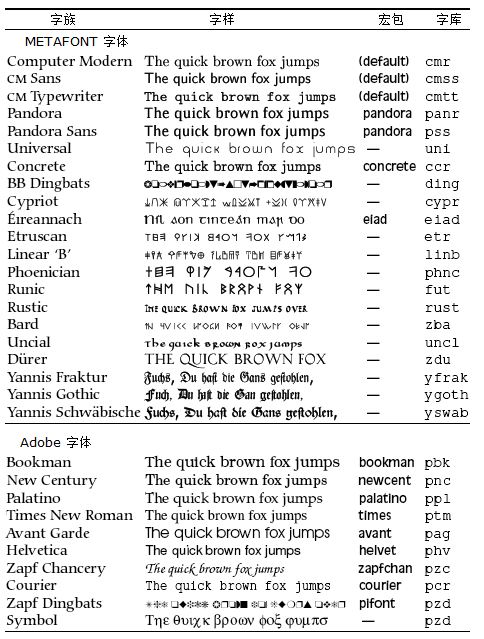
\includegraphics[scale=0.8]{font-1.jpg}
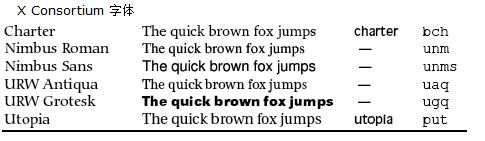
\includegraphics[scale=0.7]{font-2.jpg}
\end{figure}

\section*{NPU-Template}

https://github.com/polossk/\LaTeX{}-Template-For-NPU-Thesis 本科毕设

https://github.com/NWPUMetaphysicsOffice/Yet-Another-\LaTeX{}-Template-for-NPU-Thesis 硕博论文模版持续更新

https://github.com/zhenboliu/npu-PhD-thesis-template  硕博论文

https://github.com/lrtfm/nputhesis  硕博论文

https://github.com/NPUSCG/npu-dissertation-proposal 选题报告

https://github.com/kidozh/\LaTeX{}-Template-For-NPU-Thesis  硕博论文

\section{论文模版}

\LaTeX{}模板中包含了.tex、.cls、.bib、.bst、.eps等文件。.tex文件为\LaTeX{}的源文件,.cls文件是\LaTeX{}的样式文件,.bib文件是参数文件数据库,.bst文件是bibtex处理参考文献后生成的格式,即定义参考文献的排版效果,.eps文件是\LaTeX{}插入的图片文件。





\end{document}